% Clase del documento
\documentclass[12pt,twoside,titlepage]{report}





%%%%%%%%%%%%%%%%%%%%%%% Paquetes %%%%%%%%%%%%%%%%%%%%%%%

\usepackage[a4paper,bindingoffset=3mm,bottom=35mm]{geometry}


% Usad \usepackage[dvips]{graphicx} o \usepackage[pdftex]{graphicx} (no ambos)
%\usepackage[dvips]{graphicx} %%% para LaTeX. Las figuras deben estar en formato eps

\usepackage[colorlinks=true,pdftex]{hyperref}   %%% Opcional. Para incluir marcadores y enlaces en el pdf
\usepackage[pdftex]{graphicx}  %%% para pdflatex. Las figuras pueden estar en pdf, jpg, svg y otros formatos


\usepackage[spanish]{babel}


%\usepackage[latin1]{inputenc} % Usad en WinEdt/MikTex
\usepackage[utf8]{inputenc} % Usad en overleaf

%\usepackage[T1]{fontenc}


% Algunos paquetes útiles

\usepackage{amsmath,amssymb}
\usepackage{hyperref}
\usepackage{color}
\usepackage{afterpage}
\usepackage{paralist}
\usepackage{array}
\usepackage{enumerate}
\usepackage{paralist}
\usepackage{enumitem}
\usepackage{float}
\usepackage{setspace}
\usepackage{listings}
\usepackage{algorithm}
\usepackage{algorithmic}
\usepackage{fancyhdr}
\usepackage{rotating}
\usepackage{multirow}


% Otros paquetes

\usepackage{quotchap}
\usepackage{lipsum}

%%%%%%%%%%%%%%%%%%%%%%%%%%%%%%%%%%%%%%%%%%%%%%%%%%%%%%%%






%%%%%%%%%%%%%%%%%%%%%%% Definiciones básicas %%%%%%%%%%%%%%%%%%%%%%%

\newcommand{\nombreautor}{Oscar Nydza Nicpoñ}
\newcommand{\nombretutor}{Juan Manuel Serrano Hidalgo}
\newcommand{\titulotrabajo}{Comparativa entre las API de Spark en Scala y Python}
\newcommand{\escuela}{Escuela Técnica Superior\\de Ingeniería Informática}
\newcommand{\escuelalargo}{Escuela Técnica Superior de Ingeniería Informática}
\newcommand{\universidad}{Universidad Rey Juan Carlos}
\newcommand{\fecha}{Fecha}
\newcommand{\grado}{Grado en Ingeniería de Computadores}
\newcommand{\curso}{Curso 2021-2022}
\newcommand{\logoUniversidad}{logoURJC.pdf} % logoURJC.eps
\newcommand{\quotes}[1]{``#1''}

%%%%%%%%%%%%%%%%%%%%%%%%%%%%%%%%%%%%%%%%%%%%%%%%%%%%%%%%%%%%%%%%%%%%






%%%%%%%%%%%%%%%%%%%%%%%%% Otras definiciones %%%%%%%%%%%%%%%%%%%%%%%%%%

% Definiciones de colores (para hidelinks)
\definecolor{BlueLink}{rgb}{0.165,0.322,0.745}
\definecolor{PinkLink}{rgb}{0.8,0.22,0.5}
\definecolor{gray}{rgb}{0.6,0.6,0.6}


% Enlaces
\hypersetup{hidelinks,pageanchor=true,colorlinks,citecolor=PinkLink,urlcolor=black,linkcolor=BlueLink}


\newcommand\blankpage{%
    \newpage
    \null
    \thispagestyle{empty}%
    %\addtocounter{page}{-1}%
    \newpage}


% Texto referencias
\addto{\captionsspanish}{\renewcommand{\bibname}{Bibliografía}}

% Texto Índice de tablas
\addto\captionsspanish{
\def\tablename{Tabla}
\def\listtablename{\'{I}ndice de tablas}
}


\floatname{algorithm}{Algoritmo}

\newfloat{algorithm}{t}{lop}


%\newenvironment{pseudocodigo}[1][htb]
%  {\renewcommand{\algorithmcfname}{Pseudocódig}% Update algorithm name
%   \begin{algorithm}[#1]%
%  }{\end{algorithm}}
  
%%%%%%%%%%%%%%%%%%%%%%%%%%%%%%%%%%%%%%%%%%%%%%%%%%%%%%%%%%%%%%%%%%%%





%%%%%%%%%%%%%%%%%%%%%%% Estilo de código (en Python) %%%%%%%%%%%%%%%%%%%%%%%

\definecolor{bg}{rgb}{0.95,0.95,0.95}
\definecolor{mydeepteal}{rgb}{0.16,0.22,0.23}
\definecolor{myteal}{rgb}{0.31,0.44,0.46}
\definecolor{mymediumteal}{rgb}{0.41,0.58,0.60}

\DeclareFixedFont{\ttb}{T1}{txtt}{bx}{n}{12} % for bold
\DeclareFixedFont{\ttm}{T1}{txtt}{m}{n}{12}  % for normal


%\newcommand*{\FormatDigit}[1]{\textcolor{mydeepteal}{#1}}
\newcommand*{\FormatDigit}[1]{\textcolor{black}{#1}}

% Python style for highlighting
\newcommand\mypythonstyle{\lstset{
language=Python,
basicstyle=\ttfamily\small,
%basicstyle=\linespread{1.0}\footnotesize\ttm,
otherkeywords={self},             % Add keywords here
keywordstyle=\bfseries\ttfamily\color{myteal},
%keywordstyle=\ttb\color{myteal},
commentstyle=\itshape\color{myteal},
stringstyle=\color{mydeepteal},
emph={MyClass,__init__},          % Custom highlighting
emphstyle=\ttb\color{mydeepteal},    % Custom highlighting style
% Any extra options here
showstringspaces=false,            %
backgroundcolor=\color{bg},
rulecolor = \color{bg},
%identifierstyle=\color{deepgreen},
breaklines=true,
numbers=left,
numbersep=5pt,
numberstyle=\tiny,
tabsize=4,
xleftmargin=1em,
frame = single,
framesep = 3pt,
framextopmargin=0pt,
framexbottommargin=0pt,
framexleftmargin=0pt,
framexrightmargin=0pt,
fontadjust=true,
basewidth=0.55em, % compactness of code
upquote=true,
}}

% Python environment
\lstnewenvironment{mypython}[1][]
{
\mypythonstyle
\lstset{#1}
}
{}

\newcommand\mypythonstylenormalinline{\lstset{
language=Python,
basicstyle=\ttfamily\normalsize,
%basicstyle=\linespread{1.0}\footnotesize\ttm,
otherkeywords={self},            % Add keywords here
keywordstyle=\bfseries\ttfamily\color{myteal},
%keywordstyle=\ttb\color{myteal},
commentstyle=\itshape\color{mymediumteal},
stringstyle=\color{mydeepteal},
emph={MyClass,__init__},          % Custom highlighting
emphstyle=\ttb\color{mydeepteal},    % Custom highlighting style
% Any extra options here
showstringspaces=false,            %
backgroundcolor=\color{bg},
rulecolor = \color{bg},
%identifierstyle=\color{deepgreen},
breaklines=false,
numbers=left,
numbersep=5pt,
numberstyle=\tiny,
tabsize=4,
xleftmargin=0em,
frame = single,
framesep = 3pt,
framextopmargin=0pt,
framexbottommargin=0pt,
framexleftmargin=0pt,
framexrightmargin=0pt,
fontadjust=true,
%basewidth=0.55em, % compactness of code
upquote=true,
}}

\newcommand\mypythoninline[1]{{\mypythonstylenormalinline\lstinline!#1!}}

%%%%%%%%%%%%%%%%%%%%%%%%%%%%%%%%%%%%%%%%%%%%%%%%%%%%%%%%%%%%%%%%%%%%%%%%%%%%%%

\usepackage{listings}

% "define" Scala
\lstdefinelanguage{scala}{
  morekeywords={abstract,case,catch,class,def,%
    do,else,extends,false,final,finally,%
    for,if,implicit,import,match,mixin,%
    new,null,object,override,package,%
    private,protected,requires,return,sealed,%
    super,this,throw,trait,true,try,%
    type,val,var,while,with,yield},
  otherkeywords={=>,<-,<\%,<:,>:,\#,@},
  sensitive=true,
  morecomment=[l]{//},
  morecomment=[n]{/*}{*/},
  morestring=[b]",
  morestring=[b]',
  morestring=[b]"""
}

\usepackage{color}
\definecolor{dkgreen}{rgb}{0,0.6,0}
\definecolor{gray}{rgb}{0.5,0.5,0.5}
\definecolor{mauve}{rgb}{0.58,0,0.82}

\lstset{frame=tb,
  language=scala,
  aboveskip=3mm,
  belowskip=3mm,
  showstringspaces=false,
  columns=flexible,
  basicstyle={\small\ttfamily},
  numbers=none,
  numberstyle=\tiny\color{gray},
  keywordstyle=\color{blue},
  commentstyle=\color{dkgreen},
  stringstyle=\color{mauve},
  frame=single,
  breaklines=true,
  breakatwhitespace=true
  tabsize=3
}


%%%%%%%%%%%%%%%%%%%%%%%%%%%% Comandos definidos por el autor 

\newcommand{\transpuesta}{\mbox{\tiny $\mathsf{T}$}}








%%%%%%%%%%%%%%%%%%%%%%%%%%%%%%%%%%%%%%%%%%%%%%%%%%%%%%%%%%%%%%%%%%%%%%%
%                           Inicio del documento                       
%%%%%%%%%%%%%%%%%%%%%%%%%%%%%%%%%%%%%%%%%%%%%%%%%%%%%%%%%%%%%%%%%%%%%%%


\begin{document}

\pagestyle{plain}




%%%%%%%%%%%%%%%%%%%%%%%%%%%%%%%%%%%% Portada %%%%%%%%%%%%%%%%%%%%%%%%%%%%%%%%%%

%\pagenumbering{gobble}
%\pagenumbering{arabic}

% Universidad, Facultad
\begin{titlepage}
\selectlanguage{spanish}


% logo
\begin{center}
    \includegraphics[scale=0.7]{\logoUniversidad}
\end{center}

\bigskip

\begin{center}
\begin{LARGE}
\escuela \\
\end{LARGE}
\end{center}

\bigskip
\bigskip

% Grado
\begin{center}
\begin{large}
\textbf{\grado}\\
\end{large}
\end{center}

% Curso
\begin{center}
\begin{large}
\textbf{\curso}\\
\end{large}
\end{center}

\bigskip

\textbf{\begin{center}
\begin{large}
\textbf{Trabajo Fin de Grado}
\end{large}
\end{center}}

\bigskip
\bigskip
\bigskip

% Nombre del TFG
\begin{center}
\textbf{\begin{large}
\MakeUppercase{\titulotrabajo}\\
\end{large}}
\end{center}

% Nombre del autor
\vspace{\fill}
\begin{center}
\textbf{Autor: \nombreautor}\\ \smallskip
% Tutor
\textbf{Tutor: \nombretutor}\\
% Añadir segundo tutor si hubiera


\bigskip

% Fecha
%\textbf{\fecha}\\
\end{center}
\end{titlepage}


%%%%%%%%%%%%%%%%%%%%%%%% Opcional %%%%%%%%%%%%%%%%%%%%%%
%\blankpage

%\thispagestyle{empty}
%\begin{center}

% Nombre del trabajo
%\textbf{\begin{large}
%\MakeUppercase{\titulotrabajo}\\*
%\end{large}}
%\vspace*{0.2cm}
%\vspace{5cm}

% Nombre del autor y del tutor
%\large Autor: \nombreautor \\* \medskip
%\large Tutor: \nombretutor \\*

%\vfill

% Escuela, universidad y fecha
%\escuelalargo \\ \smallskip
%\universidad \\
%\vspace{1cm}
%\fecha \\

%\clearpage

%\end{center}
%%%%%%%%%%%%%%%%%%%%%%%%%%%%%%%%%%%%%%%%%%%%%%%%%%%%%%%%

\hypersetup{pageanchor=true}

\normalsize
\afterpage{\blankpage} % Se deben añadir página en blanco para que lo capítulos de la memoria o estas secciones introductorias empiecen en páginas impares

%%%%%%%%%%%%%%%%%%%%%%%%%%%%%%%%%%%%%%%%%%%%%%%%%%%%%%%%%%%%%%%%%%%%%%%%%%%%%%%





% Estilo de párrafo de los capítulos
\setlength{\parskip}{0.75em}
\renewcommand{\baselinestretch}{1.25}
% Interlineado simple
\spacing{1}

\pagenumbering{Roman}
\setcounter{page}{2}


%%%%%%%%%%%%%%%%%%%%%%%%% Agradecimientos o dedicatoria %%%%%%%%%%%%%%%%%%%%%%%%%%%

\chapter*{Agradecimientos}

Breves agradecimientos o dedicatoria.

\afterpage{\blankpage}

%%%%%%%%%%%%%%%%%%%%%%%%%%%%%%%%%%%%%%%%%%%%%%%%%%%%%%%%%%%%%%%%%%%%%%%%%%%%%%%%%%%






%%%%%%%%%%%%%%%%%%%%%%%%%%%%%%%%%%%% Resumen %%%%%%%%%%%%%%%%%%%%%%%%%%%%%%%%%%%%%%

\chapter*{Resumen}

Breve resumen del Trabajo de Fin de Grado (TFG). Recomendable entre 250-300 palabras, conteniendo los principales objetivos y resultados derivados del mismo.

\mbox{} \bigskip

\noindent \textbf{Palabras clave}:
\begin{compactitem}
    \item Python
    \item Ciberseguridad
    \item Aprendizaje automático (pueden ser varias)
    \item $\ldots$
\end{compactitem}

\afterpage{\blankpage}

%%%%%%%%%%%%%%%%%%%%%%%%%%%%%%%%%%%%%%%%%%%%%%%%%%%%%%%%%%%%%%%%%%%%%%%%%%%%%%%%%%%





%%%%%%%%%%%%%%%%%%%%%%%%%%%%%%%%%%%% Índices %%%%%%%%%%%%%%%%%%%%%%%%%%%%%%%%%%%%

% Estilo de párrafo de los Índices
\setlength{\parskip}{1pt}
\renewcommand{\baselinestretch}{1}
\renewcommand{\contentsname}{Índice de contenidos}


% Índice de contenidos
\tableofcontents
\afterpage{\blankpage}

% Índice de tablas (OPCIONAL)
%\listoftables
%\afterpage{\blankpage}
%\addcontentsline{toc}{chapter}{\noindent \listtablename}

% Índice de figuras (OPCIONAL)
\listoffigures
\afterpage{\blankpage}
\addcontentsline{toc}{chapter}{\listfigurename}

% Índice de códigos/algoritmos (OPCIONAL).   El término "Códigos" se puede cambiar por "Métodos", "Funciones", "Algoritmos", etc.
\renewcommand\lstlistlistingname{Códigos}
\renewcommand\lstlistingname{Código}
\renewcommand\lstlistlistingname{Índice de códigos}

\lstlistoflistings
\afterpage{\blankpage}
\addcontentsline{toc}{chapter}{\lstlistlistingname}


% En este documento (de momento) no se ha considerado incluir un índice de algoritmos/pseudocódigos, como el que aparece en \ref{AdditionalLouvain}

%%%%%%%%%%%%%%%%%%%%%%%%%%%%%%%%%%%%%%%%%%%%%%%%%%%%%%%%%%%%%%%%%%%%%%%%%%%%%%%%%%%





%%%%%%%%%%%%%%%%%%%%%%% Cabeceras y pies de página (Opcional) %%%%%%%%%%%%%%%%%%%%%%%

%\setlength{\headheight}{15.2pt}
\pagestyle{fancy}


\renewcommand{\chaptermark}[1]{\markboth{Capítulo \thechapter.\ #1}{}}

\pagestyle{fancy}
\fancyhf{}
\fancyhead[LO]{\leftmark}
\fancyhead[RO]{}
\fancyhead[RE]{\nouppercase\rightmark}
\fancyhead[LE]{}
\fancyfoot[C]{\thepage}

%%%%%%%%%%%%%%%%%%%%%%%%%%%%%%%%%%%%%%%%%%%%%%%%%%%%%%%%%%%%%%%%%%%%%%%%%%%%%%%%%%%%






%%%%%%%%%%%%%%%%%%%%%%%%%%%%%% Capítulos de la memoria %%%%%%%%%%%%%%%%%%%%%%%%%%%%%



% Capítulo 1
\chapter{Introducción}
\newpage

%%%%%%%%%%%%%%%%%%%%%%%%%%%%%%%%%%%%%%%%%%%%%%%%%%%%%%%%%%%%%%%%%%%%%%%%%%

% Estilo resto de páginas
\pagestyle{fancy}


% Estilo de párrafo de los capítulos
\setlength{\parskip}{0.75em}
\renewcommand{\baselinestretch}{1.25}
% Interlineado simple
\spacing{1}
% Numeración contenido
\pagenumbering{arabic}
\setcounter{page}{1}

%%%%%%%%%%%%%%%%%%%%%%%%%%%%%%%%%%%%%%%%%%%%%%%%%%%%%%%%%%%%%%%%%%%%%%%%%%



Se puede añadir texto antes de empezar la primera sección.


\section{Contexto y alcance}

Contexto. Situar al lector. Objetivo general y alcance del trabajo.


\section{Estructura del documento}

La estructura del TFG no es fija. El tutor indicará una estructura adecuada dependiendo del trabajo concreto.

Se puede incluir dentro de cada apartado secciones adicionales. La copia en papel de la memoria del TFG será encuadernada en pasta dura de color azul (p.e. encuadernación tipo chanel). La portada, que puede ser una pegatina transparente, seguirá el modelo que se adjunta, que incluye el escudo y nombre de la URJC, la titulación cursada por el alumno, el curso académico, el título del TFG, el autor y el o los directores/tutores.


\subsection{Trabajos de grados en informática}

Una posible estructura de la memoria final asociada con cada TFG podría ser la siguiente (leed la normativa de TFG):
\begin{enumerate}
 \item Introducción
 \item Objetivos (incluyendo descripción del problema, estudio de alternativas y metodología empleada)
 \item Descripción informática (puede incluir especificación, diseño, implementación y pruebas).
 \item Experimentos / validación
 \item Conclusiones (incluyendo los logros principales alcanzados y posibles trabajos futuros)
 \item Bibliografía
 \item Apéndices
\end{enumerate}


\subsection{Trabajos del grado en matemáticas}

Una posible estructura de la memoria final asociada con cada TFG podría ser la siguiente:
\begin{enumerate}
 \item Introducción
 \item Objetivos (incluyendo descripción del problema, estudio de alternativas y metodología empleada)
 \item Material y métodos / Metodología / Cuerpo del trabajo (describir las metodologías empleadas en el desarrollo del TFG o el desarrollo del mismo en caso de ser un trabajo de recopilación bibliográfica sobre un tema).
 \item Resultados (opcional, dependiendo del tipo de trabajo desarrollado)
 \item Conclusiones (incluyendo los logros principales alcanzados y posibles trabajos futuros)
 \item Bibliografía
 \item Apéndices
\end{enumerate}


% \afterpage{\blankpage} % puede generar problema en índice de contenidos
% \newpage







% Capítulo 2
\chapter{Objetivos}
\newpage

El principal objetivo de este Trabajo de Fin de Grado realizar una comparativa entre las API de Spark de Scala y de Python. Para ello utilizaremos un conjunto de datos del dominio de la Fórmula 1 e intentaremos responder a las siguientes preguntas mediante queries como:

\begin{compactitem}
  \item Piloto más consistente en un periodo de tiempo concreto: se calculará la diferencia entre el tiempo medio de todas las vueltas de cada piloto ese periodo de tiempo en concreto y la media de sus vueltas más rápidas.
  \item Piloto más dominante en un periodo de tiempo concreto calculando valores estadísticos como el total de carreras ganadas, el total de títulos, el número de vueltas lideradas, el número de primeras posiciones en clasificación, número de vueltas rápidas, etc. Todo ello relativo a su periodo de actividad.
  \item Similar al punto anterior, pero con fabricantes. Normalmente cada fabricante tiene varios pilotos, así que se tomarán como valor la media de todos los pilotos en cada métrica.
  \item En base a lo anterior, cuál ha sido el peor año de esa marca en ese periodo de tiempo teniendo en cuenta resultados de carrera, problemas de fiabilidad y paradas en boxes.
  \item Análisis de temporada por pilotos y constructores: se calcularán diversas medidas estadísticas para cada piloto o fabricante (utilizando la media de los valores de los pilotos en caso del fabricante). Por ejemplo, el total de podios, el porcentaje de carreras en las que se ha acabado en podio, la media de posiciones perdidas y ganadas por carrera, el número de vueltas lideradas, etc.
  \item Temporada más interesante para el espectador, teniendo en cuenta métricas como el número de adelantamientos, accidentes, retiradas de pilotos, más cambios de líder en la clasificación general, etc.
\end{compactitem}

Además de responder a estas preguntas, también me planteo los siguientes objetivos:

\begin{compactitem}
  \item Visualizar de los resultados de las queries realizadas usando Plotly. 
  \item Migrar queries desde PySpark a Scala Spark, centrando la explicación en las diferencias entre ambas APIs y en detalles a tener en cuenta al hacer una migración de este estilo.
  \item Medir y comparar el rendimiento de ambas API utilizando la Spark UI, que proporciona métricas de rendimiento en tiempo y memoria.
  \item Realizar queries a un cluster AWS EMR.
\end{compactitem}


% Capítulo 3
\chapter{Descripción Informática}
\label{chap:contenidos}
\newpage

\section{Fuentes de datos}

Como se mencionó brevemente en el apartado de Objetivos, se ha utilizado un conjunto de datos de la Fórmula 1 que fue obtenido del siguiente enlace: \href{https://www.kaggle.com/rohanrao/formula-1-world-championship-1950-2020}{click aquí}. Concretamente, este dataset tiene 13 tablas que proporcionan información sobre distintos aspectos de esta competición. Estas tablas son:

\begin{compactitem}
  \item \texttt{circuits}
  \item \texttt{constructor$\_$results}
  \item \texttt{constructor$\_$standings}
  \item \texttt{constructors}
  \item \texttt{driver$\_$standings}
  \item \texttt{lap$\_$times}
  \item \texttt{pit$\_$stops}
  \item \texttt{qualifying}
  \item \texttt{races}
  \item \texttt{results}
  \item \texttt{seasons}
  \item \texttt{status}
  \item \texttt{drivers}
\end{compactitem}

Todas estas tablas están interrelacionadas como se puede ver en el diagrama Entidad-Relación que se presenta a continuación:

\begin{figure}[H]
  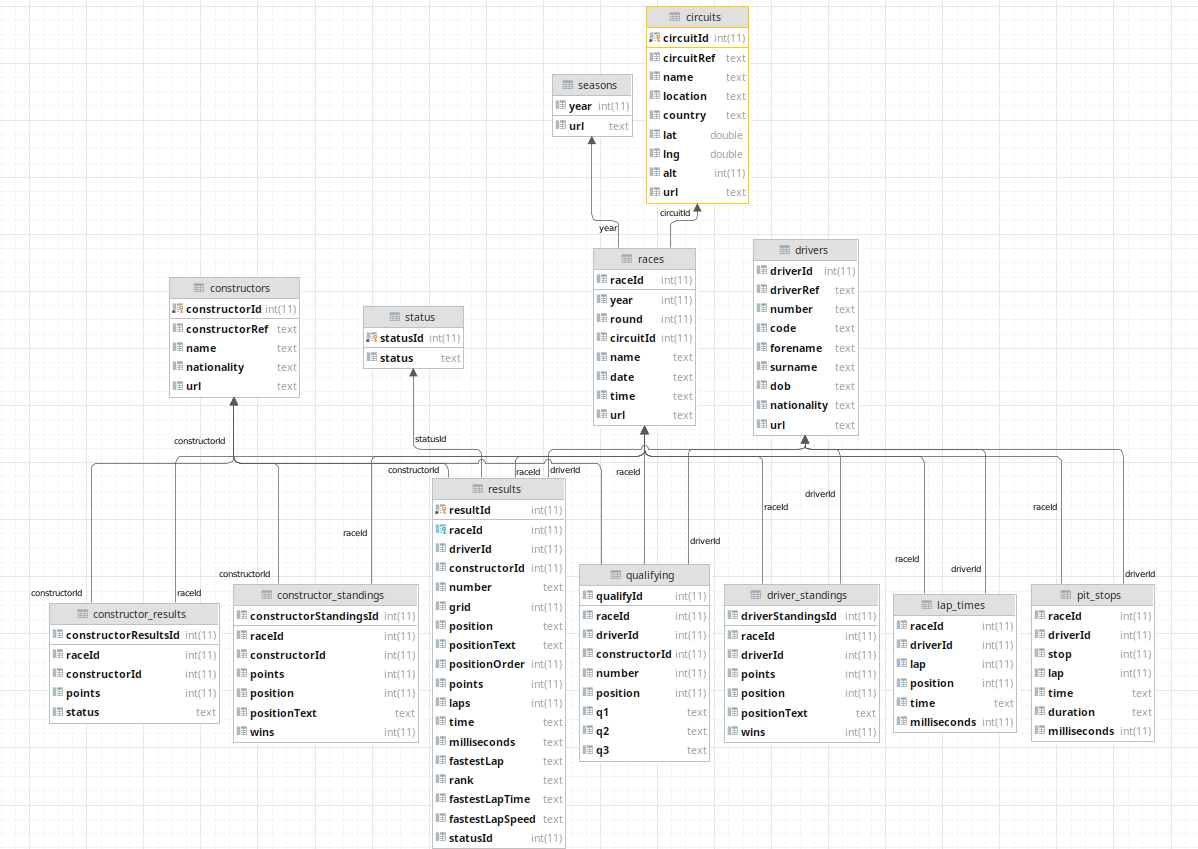
\includegraphics[scale=0.4]{dataset_visualization.png}
  \centering
  \caption{Diagrama Entidad-Relación}
  \label{fig:datavisualization}
  \centering
\end{figure}


\subsubsection{Tabla \texttt{circuits}}

Esta tabla contiene información sobre todos los circuitos en los que se ha llevado a cabo un Gran Premio. Las columnas más interesantes son el nombre del circuito, una referencia textual y la localización. 

\begin{figure}[H]
  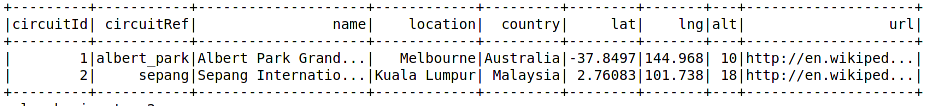
\includegraphics[scale=0.4]{circuits_table.png}
  \centering
  \caption{Tabla circuits}
  \label{fig:circuits}
  \centering
\end{figure}

\subsubsection{Tabla \texttt{constructor$\_$results}}

Esta tabla nos proporciona información sobre los resultados de las carreras en base a los constructores. 

\begin{figure}[H]
  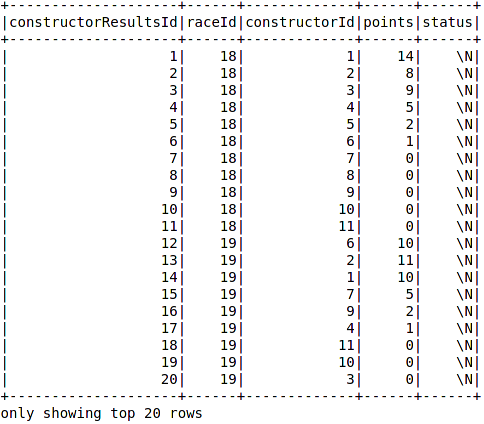
\includegraphics[scale=0.5]{constructor_results_table.png}
  \centering
  \caption{Tabla constructor$\_$results}
  \label{fig:constructorres}
  \centering
\end{figure}


\subsubsection{Tabla \texttt{constructor$\_$standings}}

Esta tabla contiene información sobre la clasificación de constructores. Como particularidad, tiene una entrada por carrera y constructor participante. Por tanto, podríamos ver cómo ha ido cambiando la clasificación de constructores a lo largo del campeonato.

Las columnas más interesantes son el identificador de la carrera, identificador del constructor, los puntos, la posición en la clasificación y las victorias hasta ese punto. 


\begin{figure}[H]
  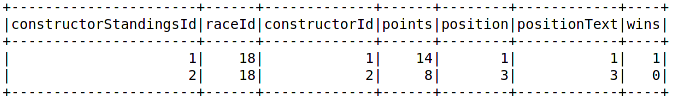
\includegraphics[scale=0.5]{constructor_standings_table.png}
  \centering
  \caption{Tabla constructor$\_$standings}
  \label{fig:constructorstands}
  \centering
\end{figure}

\subsubsection{Tabla \texttt{constructors}}

Esta tabla contiene información sobre los distintos constructores que han participado en algún campeonato mundial de Fórmula 1. Las columnas más interesantes son el id de constructor, la referencia, el nombre del constructor y la nacionalidad. 

\begin{figure}[H]
  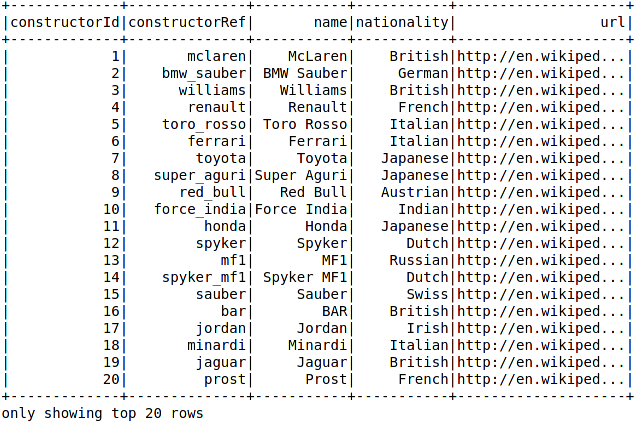
\includegraphics[scale=0.5]{constructors_table.png}
  \centering
  \caption{Tabla constructors}
  \label{fig:constructors}
  \centering
\end{figure}


\subsubsection{Tabla \texttt{driver$\_$standings}}

Similar a la tabla de clasificación de constructores, pero para pilotos. Tenemos las mismas columnas, salvo que en lugar de tener un id de constructor, lo tenemos de piloto. 


\begin{figure}[H]
  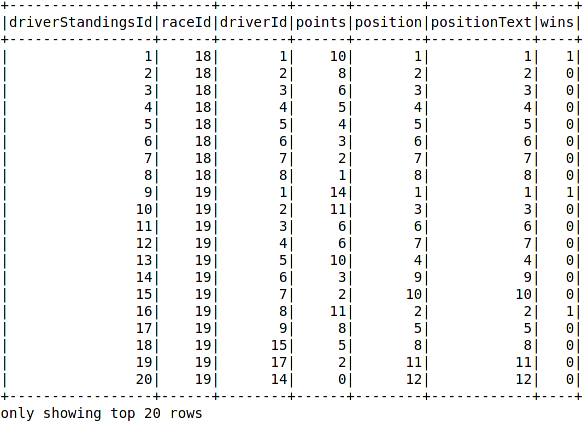
\includegraphics[scale=0.5]{driver_standings_table.png}
  \centering
  \caption{Tabla driver$\_$standings}
  \label{fig:drivstands}
  \centering
\end{figure}


\subsubsection{Tabla \texttt{lap$\_$times}}

Esta tabla es una de las más interesantes, ya que nos da todos los tiempos de vuelta de todos los pilotos desde que hay registros. Esto es, desde parte de 1996 y 1997 al completo.

Las columnas más llamativas podrían ser el id de carrera, el de piloto, la vuelta en cuestión, la posición y el tiempo en milisegundos. 

\begin{figure}[H]
  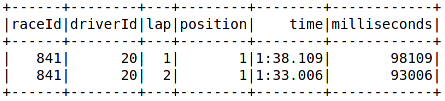
\includegraphics[scale=0.5]{lap_times_table.png}
  \centering
  \caption{Tabla lap$\_$times}
  \label{fig:laptimestab}
  \centering
\end{figure}

\subsubsection{Tabla \texttt{pit$\_$stops}}

Esta tabla contiene información de las paradas en boxes. Las columnas más interesantes son los id de carrera y piloto, el índice de parada (si es la primera, segunda, etc), la vuelta en la que se hace y la duración en milisegundos. 

\begin{figure}[H]
  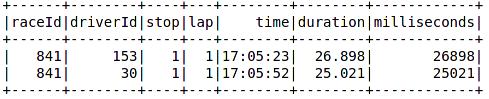
\includegraphics[scale=0.5]{pit_stop_table.png}
  \centering
  \caption{Tabla pit$\_$stops}
  \label{fig:pitstops}
  \centering
\end{figure}

\subsubsection{Tabla \texttt{qualifying}}

Esta tabla nos da información sobre los resultados de todas las rondas de clasificación. La columnas más interesantes son la posición final y los tiempos en Q1, Q2 y Q3. 

\begin{figure}[H]
  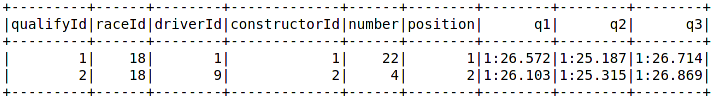
\includegraphics[scale=0.4]{qualifying_table.png}
  \centering
  \caption{Tabla qualifying}
  \label{fig:quali}
  \centering
\end{figure}


\subsubsection{Tabla \texttt{races}}

Esta tabla contiene información sobre todas las carreras celebradas en la historia de la competición. Contiene columnas como el id del circuito, el nombre del Gran Premio, la fecha y el año en el que se celebró. Esta última quizá sea la más útil de todo el dataset, ya que es la única forma de filtrar las carreras o los resultados por temporada. 

\begin{figure}[H]
  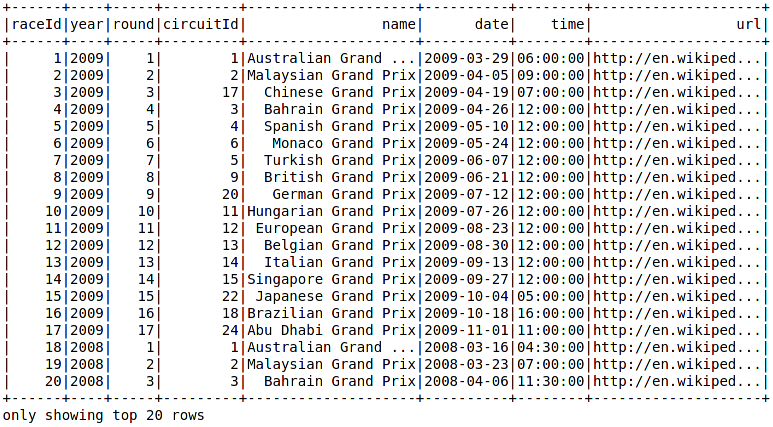
\includegraphics[scale=0.4]{races_table.png}
  \centering
  \caption{Tabla races}
  \label{fig:races}
  \centering
\end{figure}

\subsubsection{Tabla \texttt{results}}

Esta tabla es similar a la de resultados por constructor, pero para pilotos. Es la tabla más completa de todas, ya que nos proporciona una entrada por piloto y carrera con información relevante de cómo se ha desarrollado la misma. Las columnas más interesantes pueden ser la posición de salida y la posición final, los puntos ,las vueltas dadas, la vuelta más rápida, la velocidad más rápida y, en el caso de que haya habido algún incidente, el id del estado. 

\begin{figure}[H]
  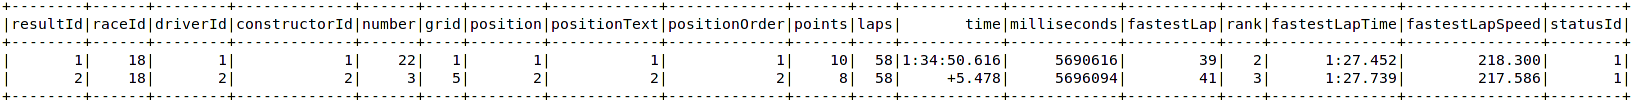
\includegraphics[scale=0.27]{results_table.png}
  \centering
  \caption{Tabla results}
  \label{fig:resultstab}
  \centering
\end{figure}

\subsubsection{Tabla \texttt{seasons}}

Quizá se trate de la tabla menos útil, ya que solamente contiene una columna con el año y otra con una url a un artículo de Wikipedia para cada entrada. 

\begin{figure}[H]
  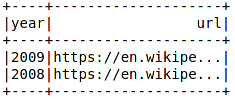
\includegraphics[scale=0.7]{season_table.png}
  \centering
  \caption{Tabla seasons}
  \label{fig:seasonstable}
  \centering
\end{figure}


\subsubsection{Tabla \texttt{status}}

Esta tabla nos da información sobre los estados en los que ha podido acabar la carrera un piloto determinado. Contiene un identificador y el estado en cuestión. 

\begin{figure}[H]
  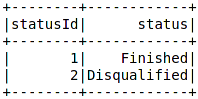
\includegraphics[scale=0.7]{status_table.png}
  \centering
  \caption{Tabla status}
  \label{fig:statustable}
  \centering
\end{figure}

\subsubsection{Tabla \texttt{drivers}}

Contiene información sobre todos los pilotos que han competido a lo largo de la historia. En concreto la información más relevante puede ser el nombre y apellido, el código, la fecha de nacimiento y la nacionalidad. 

\begin{figure}[H]
  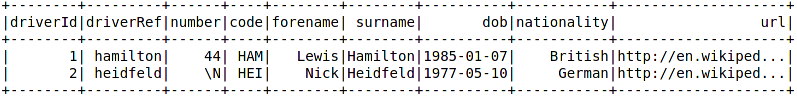
\includegraphics[scale=0.5]{driver_table.png}
  \centering
  \caption{Tabla drivers}
  \label{fig:driverstable}
  \centering
\end{figure}


\subsubsection{Tabla \texttt{drivers constructor season}} \label{drivconstseasontabexplanation}

Esta tabla no estaba originalmente en el conjunto de datos, pero resultó necesario crear una tabla nueva que relacionase cada piloto con su constructor en cada temporada. Principalmente se necesita para poder hacer comparativas entre pilotos del mismo equipo o bien globalmente o bien por temporadas. 

Esta tabla se creó a partir de la tabla \texttt{races}, que contiene la temporada y la tabla \texttt{results}, que contiene tanto el constructor como el piloto. Se hizo la intersección de estas tablas mediante la columna identificadora de la carrera. El código es el siguiente:


\begin{lstlisting}
val raceSeasonMap = spark.read.format("csv")
  .option("header", "true")
  .option("sep", ",")
  .load("../data/races.csv")
  .select("raceId", "year")

spark.read.format("csv")
  .option("header", "true")
  .option("sep", ",")
  .load("../data/results.csv")
  .join(raceSeasonMap, Seq("raceId"), "left")
  .select("year", "driverId", "constructorId")
  .dropDuplicates()
  .repartition(1)
  .write.format("csv")
  .option("header", "true")
  .save("../data/drivers_constr_season.csv")
\end{lstlisting}

Para escribir la tabla en disco, primero tenemos que utilizar \texttt{repartition} para que el resultado final quede en un solo archivo csv. Después especificamos el formato y si queremos las cabeceras o no, y proporcionamos el directorio donde queremos que quede guardado.

Finalmente la tabla contiene información tal que:

\begin{figure}[H]
  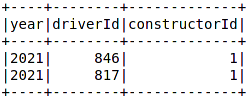
\includegraphics[scale=0.7]{driv_const_ssn_table.png}
  \centering
  \caption{Tabla auxiliar piloto-constructor-temporada}
  \label{fig:driv_const_ssn_table}
  \centering
\end{figure}



\section{Programación de queries en Scala/Spark}

\subsection{Piloto más consistente en un periodo concreto de tiempo}
En esta query intentaremos averiguar cuál ha sido el piloto más consistente en un periodo de tiempo dado. Ya que este término puede resultar ambiguo, en concreto intentaremos averiguar qué piloto tuvo una menor diferencia entre la media de sus vueltas rápidas y la media de todas las vueltas de todos los Grandes Premios de este periodo de tiempo.

Necesitaremos cruzar varias fuentes de datos para esto: 

\begin{compactitem}
  \item \texttt{races.csv}
  \item \texttt{lap$\_$times.csv}
  \item \texttt{drivers.csv}
  \item \texttt{results.csv}
\end{compactitem}

Primero de todo, queremos leer la fuente de datos \texttt{races.csv}, ya que nos permite filtrar por temporadas mediante la columna \texttt{year}. Para ello, ejecutamos las siguientes líneas de código:

\begin{lstlisting}
  val races = spark.read.format("csv")
    .option("header", "true")
    .option("sep", ",")
    .load("data/races.csv")
\end{lstlisting}

Como se puede observar, se utilizan un par de opciones de lectura. En nuestro caso, la fuente de datos contiene las cabeceras en la primera línea y cada dato está separado por una coma y por ello tenemos que especificarlo. Por último se proporciona el path relativo de la fuente de datos.

Tras esto se hace el filtro según las temporadas que se quieran usar. Para ello, ya que el periodo sobre el que se quiere obtener datos viene dado como tipo entero (ya sea en forma de lista o como un solo entero), tenemos que convertir la columna \texttt{year} a tipo entero, ya que por defecto, al no especificar el esquema a la hora de leer, Spark intenta adivinar los tipos de cada columna. Es posible que detecte esa columna como tipo entero, pero conviene asegurar haciendo la conversión de tipos. Después de esto, llevamos a cabo el filtro. Al final, para obtener este DataFrame que utilizaremos más adelante se llevan a cabo las siguientes operaciones:

\begin{lstlisting}
  val races = spark.read.format("csv")
    .option("header", "true")
    .option("sep", ",")
    .load("data/races.csv")
    .withColumn("year", col("year").cast(IntegerType))
    .where(col("year").isInCollection(seasons))
\end{lstlisting}

De este trozo de código hay que comentar un par de aspectos. Primero, la conversión de tipos, que se hace al tipo \texttt{IntegerType}, y no a \texttt{Int}, como sería intuitivo hacer. Esto es porque Spark tiene una serie de tipos concretos para el tipo \texttt{Column}. Todos ellos se encuentran en el paquete \texttt{org.apache.spark.sql.types}, y es obligatorio su uso si se utiliza la función \texttt{cast}. También cabe destacar la función de DataFrame llamada \texttt{withColumn}, que se encuentra entre las más usadas, ya que permite añadir una columna al DataFrame. Crea una columna con el nombre que recibe como primer parámetro y con el valor que recibe en el segundo. En este caso, ya que la columna \texttt{year} ya existe, se sustituye la que había anteriormente con ese nombre.

El otro aspecto a comentar es el propio filtro. Se utiliza la función \texttt{where}, que cumple el mismo propósito que su equivalente en SQL. Como parámetro recibe una condición, que en nuestro caso querríamos que fuese que \quotes{la columna \texttt{year} se encuentre entre los valores que hemos recibido}. Para ello podemos utilizar la función de columna \texttt{isInCollection}, que permite utilizar listas como filtros. En nuestro caso, \texttt{seasons} es la lista de temporadas en las que nos queremos centrar.

Resumiendo, con estas pocas líneas de código hemos obtenido todas las carreras celebradas en el rango de temporadas que necesitamos. Más adelante se utilizará para filtrar los resultados de cada piloto y obtener solamente los que nos interesan. Merecía la pena pararse en este trocito de código ya que se repite todas las queries en las que se requiere centrarse en un periodo concreto de tiempo, ya que la tabla \texttt{seasons} está, en mi opinión, incompleta y solamente contiene información de cada temporada. Es posible que más adelante añada funcionalidad a esta tabla con una columna que contenga todos los id de las carreras celebradas en esa temporada para ahorrar tiempo.

Para realizar esta consulta vamos a necesitar varios DataFrames auxiliares además del recién explicado. En concreto, necesitaremos tener una cuenta de todas las vueltas que ha dado cada piloto en el periodo de tiempo establecido, además de la tabla \texttt{drivers} para completar la información final.

Para calcular todas las vueltas que ha dado cada piloto, primero tendremos que cargar la tabla \texttt{lap$\_$times.csv} de la misma manera que hicimos anteriormente con \texttt{races.csv}. Después, le tendremos que aplicar el filtro de temporadas utilizando lo obtenido anteriormente y, por último, se hará el conteo. Todo ello se puede hacer de la siguiente manera:

\begin{lstlisting}
  val lapCount = spark.read.format("csv")
    .option("header", "true")
    .option("sep", ",")
    .load("data/lap_times.csv")
    .join(races, Seq("raceId"), "right")
    .withColumn("lapsPerDriver", count(col("lap")).over(driverWindow))
\end{lstlisting}

Como ya ha quedado claro cómo se carga información en formato CSV, paso a la siguiente línea, en la que se aplica el filtro de temporadas. Para ello hacemos la operación \texttt{join} con el DataFrame \texttt{races} obtenido anteriormente, sobre la columna \texttt{raceId} y de tipo \texttt{right}. En Spark SQL, existen varios tipos de intersecciones (join) que podemos realizar entre dos DataFrames:

\begin{compactitem}
  \item Inner Join.
  \item Full Outer Join.
  \item Left Outer Join
  \item Right Outer Join.
  \item Left Anti Join.
  \item Left Semi Join.
\end{compactitem}

Todos ellos definidos de la misma manera que en el Álgebra de Conjuntos.

Para nuestro caso particular, utilizaremos un Right Outer Join, ya que nos queremos quedar con las vueltas de las carreras definidas en \texttt{races}.

Tras esto, queremos obtener las vueltas que ha dado cada piloto en ese periodo de tiempo. Para ello, tenemos que utilizar la función \texttt{count} sobre la columna \texttt{lap}. Sin embargo, nos topamos con que, si hiciéramos eso (aparte de que el compilador no nos dejaría), necesitamos definir una ventana sobre la que operar.

Las ventanas son una parte muy útil de Spark que nos permiten centrarnos en cierta información agrupada de la forma que necesitemos. En nuestro caso, necesitamos contar las vueltas que ha dado cada piloto sin tener en cuenta las del resto y para ello necesitamos definir una ventana nueva (en nuestro caso se podría llamar \texttt{driverWindow}) que particione los datos por piloto. Esto lo hacemos de la siguiente manera:

\begin{lstlisting}
  val driverWindow = Window.partitionBy("driverId") 
\end{lstlisting}

Utilizando esta ventana, la operación \texttt{count} se llevará a cabo un conteo distinto por cada \texttt{driverId} que haya. Si particionásemos los datos según varias columnas, se llevaría a cabo la operación en cuestión según cada valor único de esas columnas en conjunto, es decir, si hay alguna variación en alguna de ellas, se toma como una operación distinta. Más adelante pondré un ejemplo de esto mismo.

Este DataFrame lo vamos a utilizar para definir cuáles son los pilotos más experimentados de este periodo de tiempo, que diremos que son los que han dado más de la media de vueltas por piloto. Para calcular esto y partiendo del DataFrame recién obtenido necesitamos conseguir dos valores: el número total de vueltas dadas entre todos los pilotos y el número de pilotos que han competido en este periodo de tiempo. Lo haremos de la siguiente manera:

\begin{lstlisting}
  val (distinctDrivers, allLaps) = lapCount
    .agg(
      countDistinct("driverID"),
      count(col("lap"))
    ).as[(BigInt, BigInt)]
    .collect()(0)
\end{lstlisting}

Estos valores los obtendré en forma de tupla, en la que el valor de la izquierda será el número de pilotos y el de la derecha el número de vueltas. Cabe centrarse en la operación \texttt{agg}, que nos permite obtener un DataFrame cuyas columnas tendrán como valor el obtenido de las operaciones que definamos. En este caso, \texttt{countDistinct} que, como su nombre indica, cuenta los valores distintos de la columna \texttt{driverId} y \texttt{count}, que realiza un conteo de todas las entradas de la columna \texttt{lap}. Con \texttt{as} le definimos el tipo de datos que queremos obtener y con \texttt{collect}, obtenemos todos los valores del DataFrame. En este caso, como solo vamos a tener una entrada, y esta va a ser la única que necesitemos, hacemos un \texttt{collect()(0)}

Para calcular la media de vueltas por piloto en este periodo de tiempo, realizamos la siguiente operación:

\begin{lstlisting}
  val avgLapsThisPeriod = allLaps.toInt / distinctDrivers.toInt
\end{lstlisting}

Con esta métrica podremos definir cuáles son los pilotos más experimentados de la siguiente manera:

\begin{lstlisting}
  val experiencedDrivers = lapCount
    .where(col("lapsPerDriver") >= avgLapsThisPeriod)
    .select("driverId")
    .distinct()
    .as[String]
    .collect()
\end{lstlisting}

Con el DataFrame obtenido anteriormente, nos quedamos con los pilotos que tengan un número de vueltas superior o igual al índice calculado. Tras esto, nos quedamos solamente con los valores distintos la columna que indica el piloto y los obtenemos en forma de \texttt{List[String]} con las dos últimas operaciones para más adelante poder filtrar según ella.

Tras esto, querremos obtener la media de todas las vueltas que ha dado cada piloto. Para ello, cargamos de nuevo la tabla \texttt{lap$\_$times.csv}, en la que tenemos una columna llamada \texttt{milliseconds} y filtramos las temporadas que nos interesan. Para asegurar, convertimos esta columna a tipo entero y hacemos la media usando la ventana que creamos antes. Eliminamos los pilotos duplicados y nos quedamos con dos columnas: identificador de piloto y la media obtenida. El código queda tal que:

\begin{lstlisting}
  val avgLapTimes = spark.read.format("csv")
    .option("header", "true")
    .option("sep", ",")
    .load("data/lap_times.csv")
    .withColumnRenamed("time", "lapTime")
    // filtro las vueltas de las carreras en el periodo de tiempo dado
    .join(races, Seq("raceId"), "right")
    .withColumn("milliseconds", col("milliseconds").cast(IntegerType))
    // media de tiempos de vuelta por piloto
    .withColumn("avgMs", avg(col("milliseconds")).over(driverWindow))
    .dropDuplicates("driverId")
    .select("driverId", "avgMs")
\end{lstlisting}


Finalmente, querríamos obtener un DataFrame que contenga dos columnas: el nombre del piloto y la diferencia ya mencionada anteriormente. Para ello, necesitamos cargar la tabla \texttt{results.csv} y dejar fuera las temporadas que no nos interesen. Esto lo haremos como ya hemos comentado antes.

Nos vamos a centrar en una de las columnas que tenemos: \texttt{fastestLapTime} que, como su nombre indica, nos da el tiempo de la vuelta más rápida de cada piloto en cada carrera. El problema es que nos lo proporciona en el formato MM:ss:mmm, donde MM son los minutos, ss los segundos y mmm los milisegundos. Necesitamos una forma de convertir esta columna a una unidad con la que podamos operar. Para este caso, lo mejor es convertir el tiempo a milisegundos.

Esta funcionalidad nos la proporcionan las UDFs (User-Defined Functions). La documentación de Spark las define como \quotes{rutinas programables por el usuario que actúan fila a fila}. Haciendo uso de ellas, podemos convertir una función que realice esta conversión que queremos a una función que actúe de la misma manera para una columna, fila a fila.

En nuestro caso vamos a tener dos funciones de este estilo: una para convertir de ese formato a milisegundos y otra que actúe de forma inversa. El código es el siguiente:


\newpage

\begin{lstlisting}
  val lapTimeToMs = (time: String) => {
    val regex = """([0-9]|[0-9][0-9]):([0-9][0-9])\.([0-9][0-9][0-9])""".r
    time match {
      case regex(min,sec,ms) => min.toInt * 60 * 1000 + sec.toInt * 1000 + ms.toInt
      case "\\N" => 180000
    }
  }: Long
\end{lstlisting}

\begin{lstlisting}
  val msToLapTime = (time: Long) => {
    val mins = time / 60000
    val secs = (time - mins * 60000) / 1000
    val ms = time - mins * 60000 - secs * 1000

    val formattedSecs = if ((secs / 10).toInt == 0) "0" + secs else secs
    // if ms = 00x -> "0"+"0"+x . if ms = 0xx -> "0"+ms
    val formattedMs =
      if ((ms / 100).toInt == 0) "0" +
        (if ((ms / 10).toInt == 0) "0" + ms else ms)
      else ms
    mins + ":" + formattedSecs + "." + formattedMs
  }: String
\end{lstlisting}

En la función \texttt{lapTimeToMs} convierto el formato de tiempo de vuelta a milisegundos. En este caso, lo hago con una expresión regular, de forma que extraigo los minutos, segundos y milisegundos de las posiciones correspondientes. Después, multiplico cada valor como corresponde y lo sumo. Es posible que, si el piloto no llegó a salir a pista, su tiempo de vuelta sea nulo, simbolizado por el string \quotes{\textbackslash\textbackslash N}. En este caso, ha decidido usar 180000 milisegundos en su lugar, o 3 minutos. Se ha decidido usar esa cifra ya que es raro que una vuelta al circuito dure más de 2 minutos y de esta manera se \quotes{penalizará} al piloto que no haya acabado la vuelta.

De forma inversa, tenemos otra función llamada \texttt{msToLapTime} que, dado un valor en microsegundos, lo convierte al formato correcto. En este caso se hace la operación inversa. Se hallan los minutos, segundos y milisegundos para más adelante formatear el texto de forma que en el caso de que un piloto hicieste un tiempo de un minuto, tres segundos y tres milisegundos, quedase formateado como \quotes{1:03:003} en lugar de \quotes{1:3:3}.

Tras esto hay que conseguir la UDF y registrarla, proceso que resulta sencillo con las siguientes instrucciones:

\newpage

\begin{lstlisting}
  val lapTimeToMsUDF = udf(lapTimeToMs)
  spark.udf.register("lapTimeToMs", lapTimeToMsUDF)
\end{lstlisting}

De esta manera podremos invocar la función \texttt{lapTimeToMsUDF}, le proporcionaremos una columna y nos de volverá otra ya procesada.

Una vez explicado esto, podemos continuar con el procesamiento del DataFrame final. Como comentamos, nos centramos en primera instancia en la columna \texttt{fastestLapTime}. Primero, debemos eliminar los valores nulos y después, todos los valores restantes los debemos convertir a milisegundos para poder operar con ellos. Esto lo podemos hacer de la siguiente manera:

\begin{lstlisting}
  spark.read.format("csv")
    .option("header", "true")
    .option("sep", ",")
    .load("data/results.csv")
    // filtro por temporada
    .join(races, Seq("raceId"), "right")
    .na.drop(Seq("fastestLapTime"))
    .withColumn("fastestLapTimeMs", lapTimeToMsUDF(col("fastestLapTime")))
\end{lstlisting}

Ya que este va a ser el DataFrame que devolvamos, podemos no guardarlo en ninguna variable y devolverlo directamente. Como viene siendo habitual, cargamos la tabla y filtramos las carreras. Después, con la función \texttt{na.drop}, eliminamos los valores nulos de la columna \texttt{fastestLapTime}. Si quisiéramos eliminar los valores nulos de varias columnas, bastaría con pasarle más nombres de columnas dentro de la lista que recibe.

Tras esto, para conseguir la columna con los milisegundos usamos \texttt{withColumn}, que recibe como nombre \texttt{fastestLapTimeMs} y como valor la conversión de la columna \texttt{fastestLapTime}, usando para ello la UDF que hemos definido.

Una vez hecho esto, aprovechamos la ventana que definimos anteriormente para hacer la media de las vueltas más rápidas de cada piloto tal que:

\begin{lstlisting}
  .withColumn("avgFastestLapMs", avg(col("fastestLapTimeMs")).over(driverWindow))
\end{lstlisting}

Ya que tendremos entradas de pilotos duplicadas, las eliminamos con la siguiente operación:

\begin{lstlisting}
  .dropDuplicates("driverId")
\end{lstlisting}

Una vez hecho esto, necesitamos la media de todas las vueltas dadas por cada piloto, que tenemos guardadas en la variable \texttt{avgLapTimes}. Tendremos que hacer una intersección sobre la columna \texttt{driverId}, pero en este caso de tipo \texttt{left}, ya que queremos completar la información que ya tenemos.

Recordemos que nuestro objetivo es obtener la diferencia entre la media de vueltas rápidas y la media de todas las vueltas. El símbolo que tenga realmente no nos interesa, ya que resulta evidente que el piloto irá más rápido en las vueltas rápidas que en la media de vueltas, pero aún así utilizaremos el valor absoluto de esta resta para eliminar signos. Ya que esta diferencia está en milisegundos, también tendremos que convertirlos al formato de tiempo de vuelta utilizando la UDF que hemos comentado anteriormente.

El código para hacer todo esto que hemos comentado sería:

\begin{lstlisting}
  .join(avgLapTimes, Seq("driverId"), "left")
  // saco el diferencial
  .withColumn("diffLapTimes", abs(col("avgMs") - col("avgFastestLapMs")).cast(IntegerType))
  // vuelvo a pasar a tiempo de vuelta
  .withColumn("avgDiff", msToLapTimeUDF(col("diffLapTimes").cast(IntegerType)))
\end{lstlisting}

En principio podríamos decir que ya tenemos lo que queremos, pero en mi opinión, no es justo tener en cuenta a pilotos que por ejemplo han corrido una sóla carrera, ya que no constituye una muestra significativa de la capacidad del piloto. Para solventar este problema podemos filtrar los pilotos no experimentados de la información que hemos obtenido utilizando la lista que llamamos \texttt{experiencedDrivers} de la siguiente manera:

\begin{lstlisting}
  .where(col("driverId").isInCollection(experiencedDrivers))
\end{lstlisting}

Una vez tenemos datos de todos los pilotos que nos interesan, pasamos a formatear la tabla que vamos a devolver. En concreto, sería interesante tener en una columna el nombre y apellido del piloto y en otra el diferencial calculado.

Para ello, tenemos que hacer otra intersección con la tabla \texttt{drivers} y concatenar el nombre y el apellido del piloto. Tras esto, nos quedamos con las columnas que nos interesan y ordenamos la tabla según el diferencial calculado de menor a mayor.

Al final, el código para obtener este DataFrame final quedaría tal que:

\vfil \break

\begin{lstlisting}
  spark.read.format("csv")
    .option("header", "true")
    .option("sep", ",")
    .load("data/results.csv")
    // filtro por temporada
    .join(races, Seq("raceId"), "right")
    .na.drop(Seq("fastestLapTime"))
    // paso la vuelta rapida de tiempo por vuelta a ms
    .withColumn("fastestLapTimeMs", lapTimeToMsUDF(col("fastestLapTime")))
    // saco la media de vueltas rapidas
    .withColumn("avgFastestLapMs", avg(col("fastestLapTimeMs")).over(driverWindow))
    .dropDuplicates("driverId")
    .join(avgLapTimes, Seq("driverId"), "left")
    // saco el diferencial
    .withColumn("diffLapTimes", abs(col("avgMs") - col("avgFastestLapMs")).cast(IntegerType))
    // vuelvo a pasar a tiempo de vuelta
    .withColumn("avgDiff", msToLapTimeUDF(col("diffLapTimes").cast(IntegerType)))
    // filtro pilotos "experimentados"
    .where(col("driverId").isInCollection(experiencedDrivers))
    // concateno el nombre y apellido de los pilotos
    .join(drivers, "driverId")
    .withColumn("driver", concat(col("forename"), lit(" "), col("surname")))
    .select("driver", "avgDiff")
    .orderBy("avgDiff")
\end{lstlisting}

\newpage


\subsection{Dominio de fabricantes en la década de los 90}

Con esta query se pretende hallar qué fabricante ha sido el más dominante en la década de los 90. En concreto intentaremos hallar el número de mundiales ganados y el número de carreras ganadas.

Se usarán las siguientes fuentes de datos:
\begin{compactitem}
  \item \texttt{races.csv}
  \item \texttt{constructor$\_$standings.csv}
  \item \texttt{constructors.csv}
\end{compactitem}

Al igual que en la query anterior, si queremos fijar nuestra atención en un periodo de tiempo, tenemos que hacerlo filtrando la columna \texttt{year} de la tabla \texttt{races.csv}. En este caso, necesitamos todas las carreras entre el año 1990 y el año 1999.

Una vez obtenidas todas las carreras de la década, tenemos que obtener la última carrera de cada temporada. Esto es debido a que en \newline\texttt{constructor$\_$standings.csv} tenemos la clasificación resultante al final de cada carrera. Para ello, usaremos crearemos una ventana en la que particionaremos los datos por año y que usaremos con la función \texttt{max()} sobre la columna \texttt{round}, que nos indica el índice de la carrera, es decir, la primera carrera de la temporada tendrá \texttt{round === 1}, para crear una columna llamada \texttt{max} en la que guardaremos el índice de la última carrera de la temporada. Finalmente, filtraremos los datos para quedarnos con aquellos en los que la columna \texttt{round === max}.

Tras esto último, unimos las tabla \texttt{constructor$\_$standings.csv} con la recién obtenida para quedarnos con los resultados en las últimas carreras y filtramos según la columna \texttt{position === 1} para quedarnos con los ganadores. Teniendo esto, podemos ver también que la columna \texttt{wins} nos proporciona el número de victorias de cada escudería en esa temporada, así que, creando una ventana en la que particionemos por fabricante podemos hallar tanto la suma de victorias como el conteo de apariciones de cada una. 

Pasando ya a la presentación de los datos, se filtrarían los constructores duplicados y se ordenarían los datos según el total de campeonatos ganados primero y, en caso de empate, por número de victorias. Además, se hace un join con la tabla de constructores para obtener su nombre.

Lo interesante de esta query es que se puede usar para cualquier periodo de tiempo. Podemos averiguar por ejemplo qué fabricante ha sido el más dominante en toda la historia de la competición y qué constructor ha dominado ciertos años concretos.

\subsection{Análisis de temporada por piloto}

Esta query consiste en obtener una serie de métricas de cada piloto en una determinada temporada. Para ello, se obtiene como parámetro la temporada en cuestión, que usaremos para filtrar.

De nuevo, lo primero es obtener las distintas carreras que se han disputado en la temporada deseada. Para ello y como ya quedó explicado anteriormente, usaremos la tabla \texttt{races}, que filtraremos según la columna \texttt{year}.

Una vez obtenidas las carreras, necesitamos obtener información personal de los pilotos para más adelante sustituir su identificador numérico por el código de tres letras personal. Como siempre, cargamos la tabla de la siguiente manera:

\begin{lstlisting}
val drivers = spark.read.format("csv")
  .option("header", "true")
  .option("sep", ",")
  .load("../data/drivers.csv")
\end{lstlisting}

Tras esto, pasamos a crear las ventanas de datos que necesitaremos. En este caso, vamos a necesitar particionar los datos por piloto, por año, por piloto y carrera y de nuevo por piloto y carrera pero ordenando por vueltas. 

\begin{lstlisting}
val driverWindow = Window.partitionBy("driverId")
val seasonWindow = Window.partitionBy("year")
val driverRaceWindow = Window.partitionBy("driverId", "raceId")
val raceDriverLapWindow = driverRaceWindow.orderBy("lap")
\end{lstlisting}

Antes de continuar, necesitaremos obtener ciertos valores estadísticos relacionados con las posiciones del piloto a lo largo de la temporada. En concreto queremos obtener todas las posiciones ganadas y perdidas a lo largo de la carrera y, ya que usaríamos la misma tabla, el número y porcentaje de vueltas que ha liderado a lo largo de la temporada.

Para ello utilizaremos la tabla \texttt{lap$\_$times.csv}, que filtraremos según las carreras de la temporada con el filtro que conseguimos antes. Para realizar estos cálculos, es importante además que las columnas \texttt{lap} y \texttt{position} sean enteros, ya que vamos a hacer comparaciones y sumatorios.

Todo esto lo podemos hacer de la siguiente manera:

\begin{lstlisting}
val driverStats = spark.read.format("csv")
  .option("header", "true")
  .option("sep", ",")
  .load("../data/lap_times.csv")
  .withColumn("position", col("position").cast(IntegerType)) 
  .withColumn("lap", col("lap").cast(IntegerType)) 
  .join(races, "raceId")
\end{lstlisting}

Para calcular si un piloto ha ganado o ha perdido su posición en una vuelta, tenemos que saber cuál es su posición en la vuelta siguiente. Para ello podemos utilizar la función \texttt{lag} de la siguiente manera:

\begin{lstlisting}
.withColumn("positionNextLap", lead(col("position"), 1).over(raceDriverLapWindow))
\end{lstlisting}


Con esto podemos calcular las vueltas ganadas o perdidas en cada vuelta de la siguiente manera:

\begin{lstlisting}
.withColumn("positionsGainedLap", when(col("positionNextLap") < col("position") , abs(col("position") - col("positionNextLap"))).otherwise(0))
.withColumn("positionsLostLap", when(col("positionNextLap") > col("position"), abs(col("position") - col("positionNextLap"))).otherwise(0))
\end{lstlisting}

De esta manera, aplicando la función \texttt{abs}, que nos devuelve el valor absoluto de la columna que se pasa como argumento, conseguimos dos de las métricas que buscábamos.

Para las otras dos métricas tendremos primero que conseguir las vueltas donde el piloto lideraba la carrera. Como tenemos información de todas las vueltas que han dado todos los pilotos en la temporada, obtener esta información no resulta complicado. Para esta query se ha realizado lo siguiente:

\begin{lstlisting}
.withColumn("lapLeader", when(col("position") === 1, 1).otherwise(0))
\end{lstlisting}

Podemos entender esta columna a la que he llamado \texttt{lapLeader} como si fuera un booleano. Si el piloto ha liderado la vuelta, valdrá \texttt{1} y en caso contrario \texttt{0}. Esto resulta muy útil ya que podemos obtener el número de vueltas que un piloto ha liderado al hacer un sumatorio de todos los elementos de esta columna particionando por piloto, como se puede ver a continuación:

\begin{lstlisting}
.withColumn("lapsLed", sum(col("lapLeader")).over(driverWindow))
\end{lstlisting}

Tras esto podemos obtener el porcentaje de vueltas que un piloto ha liderado dividiendo este valor recién calculado entre el total de vueltas dadas.

\begin{lstlisting}
.withColumn("totalLaps", sum(col("lapLeader")).over(seasonWindow))
.withColumn("percLapsLed", round(col("lapsLed") / col("totalLaps"), 2))
\end{lstlisting}

Finalmente, eliminamos duplicados y presentamos el DataFrame como consideremos oportuno. En este caso, necesitaré los cuatro valores calculados, el identificador de piloto y el de carrera. Al final la query para esta tabla quedaría tal que:

\begin{lstlisting}
val driverStats = spark.read.format("csv")
  .option("header", "true")
  .option("sep", ",")
  .load("../data/lap_times.csv")

  .withColumn("position", col("position").cast(IntegerType)) 
  .withColumn("lap", col("lap").cast(IntegerType)) 
  .join(races, "raceId")

  .withColumn("positionNextLap", lead(col("position"), 1).over(raceDriverLapWindow))
  .withColumn("positionsGainedLap", when(col("positionNextLap") < col("position") , abs(col("position") - col("positionNextLap"))).otherwise(0))
  .withColumn("positionsLostLap", when(col("positionNextLap") > col("position"), abs(col("position") - col("positionNextLap"))).otherwise(0))
  .withColumn("positionsGained", sum(col("positionsGainedLap")).over(driverRaceWindow))
  .withColumn("positionsLost", sum(col("positionsLostLap")).over(driverRaceWindow))
  .withColumn("lapLeader", when(col("position") === 1, 1).otherwise(0))
  .withColumn("lapsLed", sum(col("lapLeader")).over(driverWindow))
  .withColumn("totalLaps", sum(col("lapLeader")).over(seasonWindow))
  .withColumn("percLapsLed", round(col("lapsLed") / col("totalLaps"), 2))
  .select("raceId", "driverId", "positionsGained", "positionsLost", "lapsLed", "percLapsLed")
  .dropDuplicates()
\end{lstlisting}

El siguiente paso es obtener la tabla final, y para ello partiremos de la tabla \texttt{results}. De nuevo necesitaremos convertir a entero ciertas columnas. En este caso \texttt{position}, \texttt{grid} y \texttt{points}.

Filtramos las carreras de la temporada en cuestión y ampliamos la información con la tabla \texttt{driverStats} que acabamos de obtener y \texttt{drivers}, esta última para convertir el id de piloto en su código de 3 caracteres. Todo esto lo hacemos de la siguiente manera:

\begin{lstlisting}
val results = spark.read.format("csv")
  .option("header", "true")
  .option("sep", ",")
  .load("../data/results.csv")

  .withColumn("position", col("position").cast(IntegerType))    
  .withColumn("grid", col("grid").cast(IntegerType))    
  .withColumn("points", col("points").cast(IntegerType))

  .join(races, "raceId")
  .join(driverStats, Seq("raceId", "driverId"), "left")
  .join(drivers, "driverId")  
\end{lstlisting}

Para esta query tendremos que calcular el número de puntos obtenidos por el piloto, la media de puntos, el porcentaje de puntos en relación al ganador del campeonato, el número total de podios, el porcentaje de veces que el piloto ha acabado en el podio, el diferencial entre la posición de salida y en la que termina, la media y el total de posiciones perdidas y ganadas y el número y porcentaje de vueltas lideradas.

Antes de nada tenemos que calcular 3 valores que servirán para más adelante calcular el resto de métricas. Estos son la media de puntos, la media de puntos más alta y si el piloto ha terminado en podio o no.

De forma similar a lo visto anteriormente, para ver si un piloto ha acabado en podio podemos crear una columna llamada \texttt{podium}, que valdrá \texttt{1} si el piloto acaba en las tres primeras posiciones y \texttt{0} en caso contrario.

\begin{lstlisting}
.withColumn("podium", when(col("position") === 1 || col("position") === 2 ||col("position") === 3, lit(1)).otherwise(lit(0)))
\end{lstlisting}

La media de puntos es sencilla de calcular, y la media más alta se calcula sobre el valor anterior de la siguiente manera:

\begin{lstlisting}
.withColumn("averagePoints", round(avg(col("points")).over(driverWindow), 2))
.withColumn("maxAvgPoints", max(col("averagePoints")).over(seasonWindow))
\end{lstlisting}

Una vez obtenidos estos 3 valores podemos calcular el resto. En general todos son o bien sumatorios o medias sobre ventanas de datos concretas. Para presentar los datos de manera más accesible, se redondean a dos decimales usando la funciíon \texttt{round}.

Llegados a este punto me gustaría detenerme para explicar la función \texttt{select}. A simple vista parece sencilla si la usamos como lo haríamos en SQL o como hemos hecho hasta ahora, pero existe otra manera de usarla. Si nos vamos a la definición de la función en la documentación de Spark, veremos que le podemos pasar o bien varios String o varios objetos de tipo \texttt{Column}. Si utilizamos esta función de esta última manera, se puede obtener una cierta mejora en el plan de Spark y, por lo tanto, es recomendable utilizarla así.

En este caso, he decidido mostrar cómo finalizaríamos la query usando un \texttt{select} que recibe columnas en lugar de String. 

\begin{lstlisting}
.select(
  col("code"),
  sum(col("points")).over(driverWindow).as("champPoints"),
  col("averagePoints"),
  round(col("averagePoints") / col("maxAvgPoints"),2).as("pointPercent"),
  sum(col("podium")).over(driverWindow).as("totalPodiums"),
  round(sum(col("podium")).over(driverWindow) / count(col("podium")).over(driverWindow), 2).as("podiumPercent"),
  round(avg(col("position") - col("grid")).over(driverWindow), 2).as("positionDelta"),
  round(avg(col("positionsLost")).over(driverWindow), 2).as("avgPositionsLost"),
  round(avg(col("positionsGained")).over(driverWindow), 2).as("avgPositionsWon"),
  sum(col("positionsLost")).over(driverWindow).as("totalPositionsLost"),
  sum(col("positionsGained")).over(driverWindow).as("totalPositionsWon"),
  col("lapsLed"),
  col("percLapsLed")
)
\end{lstlisting}

Como se puede observar, podemos pasarle una columna directamente o una operación sobre ciertas columnas que devuelva un objeto de tipo \texttt{Column} a la que damos nombre con \texttt{as}.

Para calcular todas estas métricas se utiliza siempre una ventana de datos que particiona por piloto, y en los que no se particiona es porque ya existe solamente una entrada por piloto.

Como queda algún registro con valor \texttt{null}, nos convendría tratar de alguna manera estos casos, ya que se pretende representar todas estas métricas gráficamente. Para ello se utilizan las funciones presentes en el paquete \texttt{na}. Hay tres funciones que cubrirán la mayoría de casos de uso que necesitemos. Estas son: \texttt{fill}, \texttt{replace} y \texttt{drop}. Su función la indica el nombre: \texttt{fill} rellena los nulos con un literal que pasamos por parámetro, \texttt{replace} sustituye los nulos según se especifique y \texttt{drop} elimina las filas que contengan nulos, con la opción de especificar en qué columnas comprueba la existencia de estos valores.

Para la función \texttt{replace} he encontrado muy útil que puede recibir como parámetro un objeto de tipo \texttt{Map}, en el que la clave será el nombre de la columna y el valor será el valor que queramos que sustituya a los nulos. Un ejemplo podría ser el siguiente: dado un DataFrame en el que tenemos tres columnas llamadas \texttt{id}, \texttt{name} y \texttt{salary}, si utilizásemos la función \texttt{na.replace()} pasándole como parámetro \texttt{Map(\quotes{name} --> \quotes{Pedro}, \quotes{salary} --> 0)} significaría que en la columna \texttt{name} los nulos pasarán a valer "Pedro" y para la columna \texttt{salary}, los valores nulos valdrán cero.

En nuestro caso, como se ha observado que los nulos aparecen cuando el piloto no tiene ninguna vuelta que haya liderado y solo en ese caso, podemos utilizar \texttt{na.fill(0)} para solventar el problema.

Tras esto solo quedaría eliminar entradas duplicadas y ordenar según la métrica que queramos mostrar gráficamente. Todo esto lo hacemos de la siguiente manera:

\begin{lstlisting}
.na.fill(0)
.dropDuplicates(Seq("code"))
.sort(col("avgPositionsLost").desc)  
\end{lstlisting}

Al final, el código completo de la query queda tal que:

\begin{lstlisting}
val results = spark.read.format("csv")
  .option("header", "true")
  .option("sep", ",")
  .load("../data/results.csv")

  .withColumn("position", col("position").cast(IntegerType))    
  .withColumn("grid", col("grid").cast(IntegerType))    
  .withColumn("points", col("points").cast(IntegerType))

  .join(races, "raceId")
  .join(driverStats, Seq("raceId", "driverId"), "left")
  .join(drivers, "driverId")

  .withColumn("podium", when(col("position") === 1 || col("position") === 2 ||col("position") === 3, lit(1)).otherwise(lit(0)))
  .withColumn("averagePoints", round(avg(col("points")).over(driverWindow), 2))
  .withColumn("maxAvgPoints", max(col("averagePoints")).over(seasonWindow))

  .select(
    col("code"),
    sum(col("points")).over(driverWindow).as("champPoints"),
    col("averagePoints"),
    round(col("averagePoints") / col("maxAvgPoints"),2).as("pointPercent"),
    sum(col("podium")).over(driverWindow).as("totalPodiums"),
    round(sum(col("podium")).over(driverWindow) / count(col("podium")).over(driverWindow), 2).as("podiumPercent"),
    round(avg(col("position") - col("grid")).over(driverWindow), 2).as("positionDelta"),
    round(avg(col("positionsLost")).over(driverWindow), 2).as("avgPositionsLost"),
    round(avg(col("positionsGained")).over(driverWindow), 2).as("avgPositionsWon"),
    sum(col("positionsLost")).over(driverWindow).as("totalPositionsLost"),
    sum(col("positionsGained")).over(driverWindow).as("totalPositionsWon"),
    col("lapsLed"),
    col("percLapsLed")
  )

  .na.fill(0)
  .dropDuplicates(Seq("code"))
  .sort(col("avgPositionsLost").desc)
\end{lstlisting}

\section{Programación de queries en PySpark}

\subsection{Mejor temporada para el espectador}
En esta query vamos a intentar averiguar cuál ha sido la temporada más interesante desde el punto de vista del espectador. Para ello se van a calcular tres métricas: el número de adelantamientos, el número de pilotos distintos que han liderado el campeonato y el número de pilotos distintos que han ganado una carrera en dicha temporada.

Ya que se van a utilizar las tablas \texttt{lap$\_$times}, \texttt{driver$\_$standings} y \texttt{results}, vamos a necesitar mapear cada \texttt{raceId}, presente en todas estas tablas, con la correspondiente temporada en la que se disputó la carrera. Para ello utilizaremos la tabla \texttt{races}, quedándonos solamente con las columnas \texttt{raceId} y \texttt{year}. El código es el siguiente:

\begin{lstlisting}
races = spark.read.format("csv")\
  .option("header", "true")\
  .option("sep", ",")\
  .load("../data/races.csv")\
  .select("raceId", "year")
\end{lstlisting}

Solamente en este trozo pequeño de código se pueden ver algunas diferencias con la API de Scala. Principalmente se ve que se tiene que añadir el carácter \texttt{\textbackslash} al final de cada línea en la que se realiza una operación sobre el DataFrame. Iremos describiendo el resto de diferencias según vayan apareciendo.

También podemos aprovechar para crear las tres ventanas de particionado que vamos a usar. Estas son las siguientes:

\begin{lstlisting}
seasonWindow = Window.partitionBy("year")
driverRaceWindow = Window.partitionBy("driverId", "raceId")
raceDriverLapWindow = Window.partitionBy("driverId", "raceId").orderBy("lap")
\end{lstlisting}

Una vez tenemos este DataFrame con una correspondencia directa entre carrera y temporada y las ventanas de particionado, podemos calcular el número de adelantamientos. Para ello hemos de cargar la tabla \texttt{lap$\_$times}, que contiene información de todas las vueltas de cada piloto.

\begin{lstlisting}
overtakes = spark.read.format("csv")\
  .option("header", "true")\
  .option("sep", ",")\
  .load("../data/lap_times.csv")\
\end{lstlisting}

Después, viendo que tanto la columna \texttt{position} como \texttt{lap} son de tipo \texttt{String}, debemos pasarlo a entero para poder operar con ellas. Por norma general si quisiéramos comprobar una igualdad con ellas, como comprobar si estamos en la segunda vuelta, no tendríamos por qué hacer esta conversión de tipos, pero como vamos a ordenar la ventana de particionado por vuelta sí es necesario. Esto es porque dados los \texttt{String} \quotes{1}, \quotes{2} y \quotes{19}, el orden de menor a mayor sería \quotes{1}, \quotes{19} y \quotes{2}. La conversión de tipos la hacemos de la siguiente manera:

\begin{lstlisting}
  .withColumn("position", F.col("position").cast(T.IntegerType()))\
  .withColumn("lap", F.col("lap").cast(T.IntegerType()))\
\end{lstlisting}

Aqui se pueden apreciar otra diferencia respecto a Scala. Por norma general, el código en PySpark suele ser mucho más explícito por la naturaleza del lenguaje. Python y Scala son opuestos en este aspecto. 

Habiendo convertido los tipos de dichas columnas, debemos completar la información de nuestro DataFrame estableciendo una correlación entre carrera y temporada. Esto lo conseguimos interseccionándolo con el DataFrame que obtuvimos anteriormente de la siguiente manera:

\begin{lstlisting}
.join(races, "raceId")\  
\end{lstlisting}

Si no se especifica, por defecto Spark realiza una intersección de tipo \quotes{inner}.

Lo siguiente que tenemos que obtener es la posición de cada piloto en la siguiente vuelta a la que se hace referencia en la fila actual. Para ello, necesitamos particionar por carrera y piloto y ordenar la ventana de datos por vuelta. En este caso utilizamos la función \texttt{lead}, que nos devuelve la columna que proporcionamos como parámetro, pero con las entradas desplazadas \quotes{hacia arriba} el número de entradas que se indique como parámetro. Es imprescindible que la ventana que utilicemos esté ordenada. En resumidas cuentas, tendríamos en la misma entrada la posición en esta vuelta y en la siguiente. Existe otra función llamada \texttt{lag} que tiene la misma funcionalidad, pero desplaza las entradas \quotes{hacia abajo}. Para ambas funciones hay que tener en cuenta que siempre habrá una entrada de la columna desplazada que contenga un valor nulo, ya sea la primera o la última.

Teniendo la información de la siguiente vuelta, podemos ver el número de adelantamientos del piloto en esa vuelta. Para ello, si la posición en la siguiente vuelta es menor que en la actual se devuelve la diferencia y en otro caso se devuelve cero.

\begin{lstlisting}
.withColumn("positionNextLap", F.lead(F.col("position"), 1).over(raceDriverLapWindow))\
.withColumn("positionsGainedLap", F.when(F.col("positionNextLap") < F.col("position") , F.abs(F.col("position") - F.col("positionNextLap"))).otherwise(0))\
\end{lstlisting}

Tras esto, se pueden agrupar los datos según la temporada y se hace el sumatorio de los adelantamientos tal que:

\begin{lstlisting}
.groupBy("year")\
.agg(F.sum(F.col("positionsGainedLap")).alias("positionsGainedSeason"))\
\end{lstlisting}

Por último, querríamos obtener la posición que ocuparía cada temporada si las ordenásemos de más adelantamientos a menos. Esto lo podemos conseguir con la función \texttt{rank}, que se utilizará sobre una ventana sin particionar y que esté ordenada únicamente por la columna que contiene el número de adelantamientos.

\begin{lstlisting}
.withColumn("rankPositionsGained", F.rank().over(Window.orderBy(F.col("positionsGainedSeason").desc())))
\end{lstlisting}

La siguiente métrica que queremos calcular es el número de líderes distintos a lo largo de cada temporada. Para ello cargamos la tabla \texttt{driver$\_$standings} en lugar de \texttt{lap$\_$times} y completamos la información de las temporadas al igual que antes. Tras esto, tendremos la clasificación al final de cada carrera, con una entrada por piloto, carrera y temporada. Como solo nos interesan los líderes, filtramos el DataFrame para quedarnos con las entradas donde \texttt{position} valga \texttt{1}

\begin{lstlisting}
winnersTroughoutSeason = spark.read.format("csv")\
  .option("header", "true")\
  .option("sep", ",")\
  .load("../data/results.csv")\
  .join(races, "raceId")\
  .where(F.col("position") == 1)\
\end{lstlisting}

Como es bastante probable que un piloto lidere el campeonato en más de un punto a lo largo de la temporada, tenemos que deshacernos de las entradas duplicadas cada temporada:

\begin{lstlisting}
.dropDuplicates(["driverId", "position", "year"])\
\end{lstlisting}

Tras esto, nuestro DataFrame contendrá solamente los distintos pilotos que han liderado el campeonato. Como lo que queremos es saber el conteo de estos pilotos para cada temporada, debemos agrupar los datos por temporada y utilizar la función \texttt{approx$\_$count$\_$distinct} sobre la columna \texttt{driverId}.

\begin{lstlisting}
.groupBy("year")\
.agg(F.approx_count_distinct(F.col("driverId")).alias("distinctLeaders"))\  
\end{lstlisting}

Tras esto, tendremos en nuestro DataFrame una entrada por cada año.

Por último, como para la métrica anterior, crearemos una columna que nos proporcione la clasificación de las temporadas en función a la métrica que acabamos de calcular:

\begin{lstlisting}
.withColumn("rankDistinctLeaders", F.rank().over(Window.orderBy(F.col("distinctLeaders").desc())))  
\end{lstlisting}

Para la última métrica que queremos calcular podemos reutilizar prácticamente entera la query anterior. La única diferencia será que se utilizará la tabla \texttt{results}. El código es el siguiente:

\begin{lstlisting}
winnersTroughoutSeason = spark.read.format("csv")\
  .option("header", "true")\
  .option("sep", ",")\
  .load("../data/results.csv")\
  .join(races, "raceId")\
  .where(F.col("position") == 1)\
  .dropDuplicates(["driverId", "position", "year"])\
  .groupBy("year")\
  .agg(F.approx_count_distinct(F.col("driverId")).alias("distinctWinners"))\
  .withColumn("rankDistinctWinners", F.rank().over(Window.orderBy(F.col("distinctWinners").desc())))
\end{lstlisting}

Una vez calculadas las tres métricas que necesitamos, debemos encontrar una manera de establecer una clasificación global teniendolas en cuenta. En este caso, se ha decidido crear una función que para cada entrada calcule la media de cada clasificación individual. De esta manera, si una temporada ha quedado primera en más adelantamientos, tercera en más líderes de la clasificación y segunda en más ganadores distintos, se haría la media de 1, 3 y 2.

Para ello usamos una función definida por el usuario, o UDF que recibirá como parámetro una lista y devolverá su media. El código es el siguiente:

\begin{lstlisting}
def averageRank(cols):
  return sum(cols) / len(cols)

averageRank = F.udf(averageRank, T.DoubleType())
\end{lstlisting}

Es importante definir el tipo de datos de la salida de la función. En este caso, queremos devolver la media como entero, ya que no nos interesan los decimales. En caso de no definir tipo de salida, se devolverá un \texttt{StringType} que puede dar problemas a la hora de ordenar más adelante.

Para concluir, queremos interseccionar las tablas de todas las métricas según la columna \texttt{year}. En este caso podemos definir el join como \texttt{inner}, ya que al hacer la media no nos interesa que haya ningún nulo, en el caso extraño de que aparezca una temporada sin alguna métrica. Después aplicamos nuestra UDF a las columnas que queremos y preparamos el DataFrame para mostrarlo por pantalla. El código es el siguiente:

\begin{lstlisting}
overtakes\
  .join(leadersTroughoutSeason, "year", "inner")\
  .join(winnersTroughoutSeason, "year", "inner")\
  .withColumn("avgRank", averageRank(F.array(F.col("rankDistinctWinners"), F.col("rankDistinctLeaders"), F.col("rankPositionsGained"))))\
  .withColumn("overallRank", F.rank().over(Window.orderBy("avgRank")))\
  .drop("rankDistinctWinners", "rankDistinctLeaders", "rankPositionsGained", "avgRank")\
  .sort("overallRank")\
  .show()  
\end{lstlisting}

\subsection{Mejor piloto de la historia}

Para averiguar cuál es el mejor piloto de la historia, debemos fijarnos en varios aspectos del piloto, como sus logros individuales, sin comparar con nadie más a la hora de hacer el cálculo y sus logros relativos a los compañeros de equipo a lo largo de su carrera.

El primer paso para programar esta query es construir varios DataFrames auxiliares. Necesitaremos una tabla que relacione la carrera con la temporada en que tuvo lugar,  otra que nos relacione el identificador de piloto con su nombre completo, una que nos proporcione información sobre qué carreras fueron las últimas de cada temporada y por último una que establezca una relación entre los pilotos que formaron un equipo en cada temporada.

Para obtener la primera de ellas se cargará la tabla \texttt{races} y nos quedaremos con las columnas \texttt{raceId} y \texttt{year}. 

\begin{lstlisting}
races = spark.read.format("csv")\
  .option("header", "true")\
  .option("sep", ",")\
  .load("../data/races.csv")\
  .select("raceId", "year")
\end{lstlisting}

Para la segunda cargaremos la tabla \texttt{drivers} y nos quedaremos con las columnas \texttt{driverId} y una concatenación de las columnas \texttt{forename} y \texttt{surname} que llamaremos \texttt{fullName}.

\begin{lstlisting}
driverInfo = spark.read.format("csv")\
  .option("header", "true")\
  .option("sep", ",")\
  .load("../data/drivers.csv")\
  .select(F.col("driverId"),
    F.concat(F.col("forename"), F.lit(" "), F.col("surname")).alias("fullName"))
\end{lstlisting}

También necesitamos obtener la última carrera de cada temporada. Para ello cargamos de nuevo la tabla \texttt{races} y convertimos la columna \texttt{round} a tipo \texttt{IntegerType}. Acto seguido, utilizamos una ventana que particione los datos según la columna \texttt{year} para obtener el máximo de la \texttt{round}. Por último, nos quedamos con las entradas donde \texttt{round} sea igual al máximo obtenido. El código es el siguiente:

\begin{lstlisting}
lastRaces = spark.read.format("csv")\
  .option("header", "true")\
  .option("sep", ",")\
  .load("../data/races.csv")\
  .withColumn("round", F.col("round").cast(T.IntegerType()))\
  .withColumn("max", F.max(F.col("round")).over(Window.partitionBy("year")))\
  .where(F.col("round") == F.col("max"))\
  .select("raceId", "year")
\end{lstlisting}


Adicionalmente, en algún momento necesitaremos filtrar pilotos para eliminar outliers. En el caso de esta query, se ha concluido que estos serán aquellos pilotos que no hayan terminado cinco carreras o más. Para ello, cargamos la tabla \texttt{results} y nos fijamos en la columna \texttt{statusId}. Si el valor es \texttt{1}, entonces quiere decir que el piloto ha pasado por meta. Para calcular el número de carreras que ha terminado, podemos crear una columna nueva que contenga un \texttt{1} si el \texttt{statusId} tiene ese valor y \texttt{0} en caso contrario.

\begin{lstlisting}
driverFilter = spark.read.format("csv")\
  .option("header", "true")\
  .option("sep", ",")\
  .load("../data/results.csv")\
  .withColumn("finished", F.when(F.col("statusId") == 1, 1).otherwise(0))\
\end{lstlisting}

Acto seguido podemos hacer un sumatorio de esta columna particionando por piloto y después filtrar los que no lleguen a cinco. Al poder tener varias entradas por piloto, usamos la función \texttt{distinct()} para deshacernos de estos valores repetidos.

\begin{lstlisting}
  .withColumn("numberOfFinishes", F.sum(F.col("finished")).over(driverWindow))\
  .where(F.col("numberOfFinishes") < 5)\
  .select("driverId")\
  .distinct()
\end{lstlisting}

Por último, como ya comentamos cómo obtener una relación entre pilotos, fabricante y temporada en la sección  \ref{drivconstseasontabexplanation}, no entraremos al detalle de cómo se obtiene y simplemente cargaremos dicha tabla con:

\begin{lstlisting}
driverConstSeasonMap = spark.read.format("csv")\
  .option("header", "true")\
  .option("sep", ",")\
  .load("../data/drivers_constr_season.csv")
\end{lstlisting}

También necesitaremos las siguientes ventanas de datos auxiliares:

\begin{lstlisting}
raceDriverLapWindow = Window.partitionBy("driverId", "raceId").orderBy("lap")
driverWindow = Window.partitionBy("driverId")
seasonWindow = Window.partitionBy("year")
teammateWindow = Window.partitionBy("year", "constructorId")
raceConstructorWindow = Window.partitionBy("raceId", "constructorId")
seasonConstructorWindow = Window.partitionBy("year", "constructorId")
driverSeasonWindow = Window.partitionBy("driverId", "year")
\end{lstlisting}


A continuación podemos pasar a la primera query, con la que trataremos de averiguar el porcentaje de temporadas en las que, a lo largo de su carrera, un ha terminado por delante de su compañero de equipo.


Para ello, primero cargaremos la tabla \texttt{driver$\_$standings}, que interseccionaremos con \texttt{lastRaces} para quedarnos con la clasificación en la última carrera de cada temporada y con \texttt{driverConstSeasonMap} para completar con la información que nos proporciona dicha tabla.

\begin{lstlisting}
driverDomination = spark.read.format("csv")\
  .option("header", "true")\
  .option("sep", ",")\
  .load("../data/driver_standings.csv")\
  .join(lastRaces, ["raceId"], "right")\
  .join(driverConstSeasonMap, ["driverId", "year"], "left")\
\end{lstlisting}

El siguiente paso es averiguar el porcentaje de puntos que cada piloto ha obtenido para el equipo en cada temporada. Para ello dividiremos los puntos obtenidos por un piloto entre el total del equipo, calculado haciendo un sumatorio de los puntos según la ventana \texttt{teammateWindow}.

Para ver si un piloto ha dominado a su compañero de equipo en una temporada en concreto, podemos usar este último valor calculado y averiguar el máximo entre los integrantes del equipo. Cuando en una entrada de la tabla tengamos que un piloto iguala en puntos a este máximo, sabremos que ha sido el dominante en esa temporada.

\begin{lstlisting}
.withColumn("teamPointsPerc", F.col("points") / F.sum(F.col("points")).over(teammateWindow))\
.withColumn("bestOfTeam", F.max(F.col("teamPointsPerc")).over(teammateWindow))\
.withColumn("dominatedTeammate", F.when(F.col("teamPointsPerc") == F.col("bestOfTeam"), 1).otherwise(0))\
\end{lstlisting}

Con este último cálculo podemos ver cuántas temporadas ha dominado cada piloto, pero es más útil para nosotros relativizarlo a la carrera de cada piloto. Por ejemplo, si un piloto compite cuatro años y domina tres de ellos, su total de temporadas dominadas será tres, mientras que el porcentaje de su carrera en la que ha dominado a su compañero de equipo es del 75\%. Esto nos es útil ya que el número de temporadas en las que un piloto compite en el deporte puede variar drásticamente, desde una sola temporada a veinte por poner alguna cifra.

Con esto en mente, podemos contar el número de temporadas en las que ha dominado y dividirlo entre el número de temporadas en las que ha competido, utilizando para ambos parámetros una ventana de datos que particione por piloto

\begin{lstlisting}
.withColumn("dominationPerc", F.round(F.sum(F.col("dominatedTeammate")).over(driverWindow) / F.count(F.col("year")).over(driverWindow) * 100, 2))\
\end{lstlisting}

Calculada esta métrica, podemos pasar a calcular el resto. Para ello primero cargamos la tabla \texttt{results} y filtramos los outliers interseccionando con la tabla \texttt{driverFilter}. Para llevar a cabo este filtrado, debemos hacer la intersección de tipo \texttt{leftanti}. También interseccionamos con la tabla \texttt{races} para obtener información sobre la temporada en la que se llevó a cabo cada carrera.

Como las columnas \texttt{position} y \texttt{grid} son de tipo \texttt{String}, debemos cambiarlas a tipo entero y tratar los nulos en ambos casos. Esto último es importante, ya que al ordenar estas columnas los nulos quedan por encima del resto. Estos nulos aparecen debido a que no todas las entradas de esta columna contienen números. En el caso de que un piloto no haya terminado la carrera aparecerá un \quotes{\texttt{$\backslash$N}}.

Para encargarnos de estos valores nulos, se puede usar la función \texttt{na.fill()}, que en este caso recibirá un diccionario cuya clave será un \texttt{String} que denote el nombre de la columna y el valor será el que queremos dar en caso de encontrar un nulo. Para este caso se ha decidido que los nulos se sustituyan por el valor \texttt{100}, ya que en ambos casos nunca ha habido una carrera con ese número de competidores, asegurando así que siempre aparecerá el último si quisiéramos ordenar de menor a mayor.

\begin{lstlisting}
teammateComparison = spark.read.format("csv")\
  .option("header", "true")\
  .option("sep", ",")\
  .load("../data/results.csv")\
  .join(driverFilter, ["driverId"], "leftanti")\
  .join(races, "raceId")\
  .withColumn("position", F.col("position").cast(T.IntegerType()))\
  .withColumn("grid", F.col("grid").cast(T.IntegerType()))\
  .na.fill({"position" : 100, "grid" : 100})\
\end{lstlisting}

Habiendo terminado con la preparación del DataFrame, podemos calcular las siguientes métricas: el porcentaje de carreras en las que un piloto ha acabado mejor que su compañero en la parrilla de salida y al acabar y el porcentaje total de temporadas en las que ha quedado mejor que el compañero de equipo igual, tanto en la parrilla de salida como al acabar. Para ello lo primero será averiguar cuándo un piloto ha acabado por delante de su compañero de equipo en una carrera. Esto lo conseguiremos sacando el mínimo valor de la columna \texttt{position} particionando sobre fabricante y carrera y comparando con la posición en la que ha terminado cada piloto.

\begin{lstlisting}
.withColumn("topPos", F.min(F.col("position")).over(raceConstructorWindow))\
.withColumn("constructorBestPos", F.when(F.col("topPos") == F.col("position"), 1).otherwise(0))\
\end{lstlisting}

Tras esto podemos calcular el porcentaje de carreras en las que cada piloto ha estado por delante de su compañero dividiendo la suma de la última columna entre el conteo de carreras en la temporada del piloto.

\begin{lstlisting}
.withColumn("topPosPerc", F.sum(F.col("constructorBestPos")).over(driverSeasonWindow) / 
F.count(F.col("raceId")).over(driverSeasonWindow) * 100)\
\end{lstlisting}

El siguiente paso será cuantificar este dominio calculando el porcentaje de carreras de la temporada en la que ha quedado por delante del resto del equipo. Para ello primero tenemos que averiguar carrera a carrera dentro del equipo quien tiene el \texttt{topPosPerc} más alto, y \quotes{marcar} cuando nuestro \texttt{topPosPerc} sea el más alto para luego ver el porcentaje de temporadas que ha dominado.

\begin{lstlisting}
.withColumn("constTopPosPerc", F.max(F.col("topPosPerc")).over(seasonConstructorWindow))\
.withColumn("driverDomConstPos", F.when(F.col("constTopPosPerc") == F.col("topPosPerc"), 1).otherwise(0))\
\end{lstlisting}

Con una serie de operaciones muy similares, podemos calcular lo mismo pero en lugar de tener en cuenta la posición en la que termina la carrera, la posición en la parrilla de salida:

\begin{lstlisting}
.withColumn("topGrid", F.min(F.col("grid")).over(raceConstructorWindow))\
.withColumn("constructorBestGridPos", F.when(F.col("topGrid") == F.col("grid"), 1).otherwise(0))\
.withColumn("topGridPerc", F.sum(F.col("constructorBestGridPos")).over(driverSeasonWindow) / 
F.count(F.col("raceId")).over(driverSeasonWindow) * 100)\
.withColumn("constTopGridPerc", F.max(F.col("topGridPerc")).over(seasonConstructorWindow))\
.withColumn("driverDomConstGrid", F.when(F.col("constTopGridPerc") == F.col("topGridPerc"), 1).otherwise(0))\
\end{lstlisting}

Como queremos quedarnos con una entrada por piloto y temporada, aplicamos un \texttt{dropDuplicates} a las columnas pertinentes.

\begin{lstlisting}
.dropDuplicates(["driverId", "year"])\	
\end{lstlisting}

Para calcular las métricas finales, haremos la media de las columnas \texttt{avgTopDom} y \texttt{avgDom}. La media de la primera columna nos dará el porcentaje de veces que ha quedado por delante de un compañero a lo largo de la carrera, tanto para la posición de salida como la de finalizado y la media de la segunda nos dará el porcentaje de temporadas en las que ha dominado a su compañero de equipo.

\begin{lstlisting}
.withColumn("avgTopPosPerc", F.avg(F.col("topPosPerc")).over(driverWindow))\
.withColumn("avgTopGridPerc", F.avg(F.col("topGridPerc")).over(driverWindow))\
.withColumn("avgPosDom", F.avg(F.col("driverDomConstPos")).over(driverWindow))\
.withColumn("avgGridDom", F.avg(F.col("driverDomConstGrid")).over(driverWindow))\
\end{lstlisting}

Por último, como solo queremos una entrada por piloto, hacemos otro \texttt{dropDuplicates} y seleccionamos las columnas que queremos que queden en el DataFrame.

\begin{lstlisting}
.dropDuplicates(["driverId"])\
.select("driverId", "avgTopPosPerc", "avgTopGridPerc", "avgPosDom", "avgGridDom")
\end{lstlisting}

Sin embargo, estas no son las únicas métricas que queremos calcular. Estamos interesados también en las siguientes:

\begin{compactitem}
	\item Posibilidad de que empiece la carrera en primera fila.
	\item Posición media de salida.
	\item Posición media al acabar la carrera.
	\item Total de poles.
	\item Porcentaje de poles relativo al número de carreras en las que se ha participado.
	\item Porcentaje de temporadas en las que ha conseguido una pole.
	\item Porcentaje de temporadas en las que ha ganado una carrera.
	\item Porcentaje de podios relativo al número de carreras en las que se ha participado.
\end{compactitem}

Primero, como viene siendo habitual, preparamos el DataFrame para los cálculos. Cargamos la tabla \texttt{results} e interseccionamos con los DataFrames \texttt{driverDomination} según las columnas \texttt{driverId} y \texttt{year} y \texttt{teammateComparison} según la columna \texttt{driverId}. En ambos casos hacemos una intersección de tipo left. También interseccionamos con \texttt{races} para añadir información sobre la temporada en la que se ha disputado cada carrera.

Por último hacemos la intersección con \texttt{driverFilter} tomando como referencia la columna \texttt{driverId}. Sin embargo, esta intersección se hará de tipo \quotes{leftanti}. Esto quiere decir que el DataFrame resultante contendrá todos los elementos que no estén en el que queremos interseccionar por la derecha.

Esta es una manera eficiente de hacer un filtro en Spark. Otra manera sería hacer un \texttt{collect()} de \texttt{driverFilter} y obtenerlo como una lista. Llegados a este punto, en lugar de hacer una intersección \quotes{leftanti}, haríamos algo como:

\begin{lstlisting}
.where(~F.col('driverId').isin(lista))
\end{lstlisting}

Sin embargo, hacer un \texttt{collect()} en Spark resulta muy costoso y por ello se ha optado por la primera opción.

De nuevo tendremos que convertir a tipo entero las columnas \texttt{grid} y \texttt{position}. El código para preparar este DataFrame es el siguiente:

\begin{lstlisting}
results = spark.read.format("csv")\
  .option("header", "true")\
  .option("sep", ",")\
  .load("../data/results.csv")\
  .join(driverFilter, ["driverId"], "leftanti")\
  .join(races, "raceId")\
  .join(driverDomination, ["driverId", "year"], "left")\
  .join(teammateComparison, ["driverId"], "left")\
  .withColumn("grid", F.col("grid").cast(T.IntegerType()))\
  .withColumn("position", F.col("position").cast(T.IntegerType()))\
\end{lstlisting}

Lo primero que podemos calcular es el porcentaje de salidas en primera fila. Para ello primero tendremos que definir una columna que valga \texttt{1} cuando estemos en primera o segunda posición y \texttt{0} en otro caso. Para calcular la métrica podemos hacer sumar la columna recién definida particionando por piloto.

\begin{lstlisting}
.withColumn("firstRowStart", F.when((F.col("grid") == 1)  | (F.col("grid") == 2), 1).otherwise(0))\
.withColumn("firstRowChance", F.round(F.sum(F.col("firstRowStart")).over(driverWindow) / F.count(F.col("firstRowStart")).over(driverWindow), 4) * 100)\
\end{lstlisting}

Lo siguiente que podemos calcular es la posición de salida y la posición al acabar media. Esto se puede hacer con las siguientes líneas de código:

\begin{lstlisting}
.withColumn("avgGridStart", F.round(F.avg(F.col("grid")).over(driverWindow), 2))\
.withColumn("avgFinish", F.round(F.avg(F.col("position")).over(driverWindow), 2))\
\end{lstlisting}

También podemos calcular el total de poles, el porcentaje de poles respecto a todas las carreras disputadas y el porcentaje de temporadas en las que ha conseguido una pole.

Para ello primero tenemos que diferenciar las poles, esto es, cuando el piloto sale primero al iniciar la carrera. Después podemos sumar todas las poles de forma global para la primera métrica y particionando por temporada también para continuar calculando las siguientes.

El porcentaje de poles respecto al número de carreras podemos obtenerlo dividiendo el total con el conteo de carreras en las que ha participado el piloto. Para calcular el porcentaje de temporadas con pole, primero debemos de nuevo definir en qué temporadas ha conseguido alguna y hacer una cuenta similar a la anterior. Sumando todas las temporadas en las que se ha conseguido y dividiendo entre el total de campeonatos disputados. El código es el siguiente:

\begin{lstlisting}
.withColumn("pole", F.when(F.col("grid") == 1, 1).otherwise(0))\
.withColumn("totalPolePositions", F.sum(F.col("pole")).over(driverWindow))\
.withColumn("polesPerSeason", F.sum(F.col("pole")).over(driverSeasonWindow))\
.withColumn("poleChance", F.round(F.col("totalPolePositions") / F.count(F.col("raceId")).over(driverWindow) * 100, 2))\
.withColumn("hasPoleThisSeason", F.when(F.col("polesPerSeason") > 0, 1).otherwise(0))\
.withColumn("percSeasonsWithPole", F.round(F.sum(F.col("hasPoleThisSeason")).over(driverWindow) / F.count(F.col("year")).over(driverWindow), 4) * 100)\
\end{lstlisting}

Querríamos también hallar estas mismas métricas, pero para victorias. Esto resulta muy similar, salvo que en lugar de usar la columna \texttt{grid}, se usa la columna \texttt{position}:

\begin{lstlisting}
 .withColumn("win", F.when(F.col("position") == 1, 1).otherwise(0))\
.withColumn("totalVictories", F.sum(F.col("win")).over(driverWindow))\
.withColumn("victoryChance", F.round(F.col("totalVictories") / F.count(F.col("win")).over(driverWindow), 4) * 100)\
.withColumn("winsPerSeason", F.sum(F.col("win")).over(driverSeasonWindow))\
.withColumn("hasWonThisSeason", F.when(F.col("winsPerSeason") > 0, 1).otherwise(0))\
.withColumn("percSeasonsWithWins", F.round(F.sum(F.col("hasWonThisSeason")).over(driverWindow) / F.count(F.col("year")).over(driverWindow), 4) * 100)\
\end{lstlisting}

También nos interesaría calcular el porcentaje de carreras en las que se ha obtenido un podio. Para ello primero definimos cuándo se ha conseguido un podio, es decir, cuando se ha terminado primero, segundo o tercero. Después y de forma muy parecida a los cálculos anteriores, podemos hacer una suma de todos los podios y dividir por el número de carreras disputadas.

\begin{lstlisting}
.withColumn("podium", F.when((F.col("position") == 1) | (F.col("position") == 2) | (F.col("position") == 3), 1).otherwise(0))\
.withColumn("podiumChance", F.round(F.sum(F.col("podium")).over(driverWindow) / F.count(F.col("podium")).over(driverWindow), 4) * 100)\
\end{lstlisting}

Por último, eliminamos la duplicidad según la columna \texttt{driverId} y seleccionamos las columnas que queremos que continúen.

\begin{lstlisting}
.dropDuplicates(["driverId"])\
.select("driverId", "firstRowChance", "avgGridStart", "avgFinish", 
"totalPolePositions", "poleChance", "percSeasonsWithPole", 
"percSeasonsWithWins", "podiumChance", "dominationPerc", 
"avgTopPosPerc", "avgTopGridPerc", "avgPosDom", "avgGridDom")
\end{lstlisting}

Para finalizar esta query, crearemos una clasificación para cada métrica que hemos calculado. Algunas de menor a mayor y otras al contrario, y aplicaremos la UDF que programamos en la query anterior para hacer la media estas clasificaciones.

\begin{lstlisting}
results\
  .withColumn("rankFRC", F.rank().over(Window.orderBy(F.col("firstRowChance").desc())))\
    ...
  .withColumn("rankGridDom", F.rank().over(Window.orderBy(F.col("avgGridDom").desc())))\
  .withColumn("stats", averageRank(
    F.array(F.col("rankFRC"),
    F.col("rankAGS"),
      ...
    F.col("rankGridDom")
    )
  ))\
\end{lstlisting}

Además, creamos una columna que clasifique la columna \texttt{stats} de menor a mayor y ordenamos el DataFrame y ya por último completamos la información del piloto, en este caso nombre y apellido, interseccionando con el DataFrame \texttt{driverInfo}.








\section{Despliegue en AWS EMR}



% Nuevo capítulo
\chapter{Experimentos / Validación}
\label{sec:expVal}
\newpage

El primer paso para llevar a cabo esta query es cargar las fuentes de datos mencionadas. Para ello necesitamos haber creado un objeto \texttt{SparkSession}. En nuestro caso, esto se hace de la siguiente manera en el objeto \texttt{Main}:

\begin{lstlisting}
  val spark: SparkSession = SparkSession
    .builder()
    .master("local[*]")
    .getOrCreate()
\end{lstlisting}

En nuestro caso con estas opciones es suficiente, ya que estamos dedicando todos los núcleos de nuestra máquina local para las tareas que vayamos a realizar. Sin embargo, existen otras opciones que podríamos añadir si fuese necesario, como un nombre para la aplicación con \texttt{.appName("Nombre")}. Un parámetro que puede resultar muy útil modificar es el de \texttt{spark.sql.broadcastTimeout}, que por defecto tiene un valor de 300 (segundos), si no tenemos muchos recursos y vemos que la aplicación para inesperadamente con una excepción que muestra el mensaje \quotes{Could not execute broadcast in 300 secs}. Para hacer esto, la creación de la \texttt{SparkSession} sería tal que:

\begin{lstlisting}
  val spark: SparkSession = SparkSession
    .builder()
    .master("local[*]")
    .config("spark.sql.broadcastTimeout", "36000")
    .getOrCreate()
\end{lstlisting}

De igual manera, si quisiéramos modificar algún parámetro distinto, lo haríamos añadiendo más modificaciones tal que: 

\begin{lstlisting}
  val spark: SparkSession = SparkSession
    .builder()
    .master("local[*]")
    .config("spark.some.config.option", "some-value")
    .config("spark.some.config.option", "some-value")
       ...
    .getOrCreate()
\end{lstlisting}

Una vez tenemos el \texttt{SparkSession} creado correctamente, podemos usarlo para leer y escribir datos en distintos formatos, como CSV o Parquet. Además, nos permitirá crear DataFrames a partir distintos de tipos de datos, como Listas o Tuplas.



\section{Análisis de requisitos no funcionales}






% Nuevo capítulo

\chapter{Conclusiones y trabajos futuros}
\newpage

En este capítulo se detallan las conclusiones derivadas del TFG y la propuesta de posibles trabajos futuros.

Las citas del texto Autor \cite{giaquinta}, Autor \cite{fortune}, Autor \cite{fortuneB}, Autor \cite{mitchell} y Autor \cite{morrey} deben ir referenciadas en la bibliografia.


\section{Texto de relleno}

\lipsum[1-18]
\blankpage









%%%%%%%%%%%%%%%%%%%%%%%%%%%%%%% Bibliografía %%%%%%%%%%%%%%%%%%%%%%%%%%%%%%%

\phantomsection
\addcontentsline{toc}{chapter}{Bibliografía}

\footnotesize{
%\bibliographystyle{hispa}
\bibliographystyle{IEEEtran}
\bibliography{bibliografia}
}



% No expandir elementos para llenar toda la página
\raggedbottom
\afterpage{\blankpage}

\newpage




%%%%%%%%%%%%%%%%%%%%%%%%%%%%%%% Apéndices %%%%%%%%%%%%%%%%%%%%%%%%%%%%%%%

\appendix

\phantomsection
\addcontentsline{toc}{chapter}{Apéndices}

\mbox{}
\vfill
\begin{center}
\begin{Huge}
\textbf{Apéndices}
\end{Huge}
\end{center}
\vfill
\mbox{}
\thispagestyle{empty}

\newpage
\mbox{}
\thispagestyle{empty}
\newpage


% Primer apéndice
\chapter{Apéndice de figuras}
\label{sec:apendice}



% Fin del documento
\end{document}
